% delete/add 'monochrome' to allow/disallow colors
\documentclass[11pt,a4paper]{article}
\usepackage[left=1in, right=1in, top=1in, bottom=1in]{geometry}
\usepackage{graphicx}
\usepackage{bm}
\usepackage{amsmath}
\usepackage{amssymb}
\usepackage{bbm}
\usepackage{mathabx}
\usepackage[tableposition=top]{caption}
\usepackage{subcaption}
\usepackage{booktabs} % for \midrule in tables
\usepackage{float}
\usepackage[final]{pdfpages}
\usepackage{listings}
\usepackage{subfiles}
\usepackage[mode=buildnew]{standalone}
\usepackage{tikz}
\usetikzlibrary{calc,arrows,patterns,intersections}
\usepackage{pgfplots}
\usepackage{xcolor}
\usepgfplotslibrary{fillbetween}
% \usepackage[abspath]{currfile}
\usepackage[colorinlistoftodos,prependcaption,textsize=tiny]{todonotes}
\usepackage{shellesc}
\usepackage{authblk}
\usepackage[symbol]{footmisc}
\usepackage{hhline}
\usepackage{hyperref}
\hypersetup{
    colorlinks=true, %set true if you want colored links
    linktoc=all,     %set to all if you want both sections and subsections linked
    linkcolor=blue,  %choose some color if you want links to stand out
}
% \usepackage[intoc]{nomencl}
\usepackage[toc]{glossaries}

\DeclareCaptionLabelFormat{andtable}{#1~#2  \&  \tablename~\thetable}

\renewcommand{\thefootnote}{\fnsymbol{footnote}}

\newcommand{\astfootnote}[1]{%
    \let\oldthefootnote=\thefootnote%
    \setcounter{footnote}{0}%
    \renewcommand{\thefootnote}{\fnsymbol{footnote}}%
    \footnote{#1}%
    \let\thefootnote=\oldthefootnote%
}

\usepackage[backend=biber,
            style=numeric, %alphabetic
            sorting=none,
            %backref=true,
            abbreviate=false,
            dateabbrev=false,
            alldates=long]{biblatex}
\renewbibmacro*{volume+number+eid}{%
    \printfield{volume}%
    %  \setunit*{\adddot}% DELETED
    \setunit*{\addnbspace}% NEW (optional); there's also \addnbthinspace
    \printfield{number}%
    \setunit{\addcomma\space}%
    \printfield{eid}
}
\DeclareFieldFormat[article]{number}{\mkbibparens{#1}}

\renewbibmacro*{in:}{%
    {\printtext{\intitlepunct}}
}

%\usepackage{natbib}
%\setcitestyle{semicolon,aysep={},yysep={,},notesep={; }}

\addbibresource{bibliography/Bibliography.bib}

\usepackage{color}   %May be necessary if you want to color links

\newcommand{\Lagr}{\mathcal{L}}
\newcommand{\Uniform}{\mathcal{U}}
\newcommand{\norm}[1]{\left\lVert#1\right\rVert}
\DeclareMathOperator{\E}{\mathbb{E}}

% \makenomenclature
\newglossary*{type1}{Nomenclature}
\newglossary*{type2}{Abbreviations}
\makeglossaries


\newglossaryentry{IS}{
    name=IS,
    description={In-sample},
    type=type1
}
\newglossaryentry{OOS}{
    name=OOS,
    description={Out-of-sample},
    type=type2
}

\begin{document}
\title{
    %A Pioneering Market Framework for Promoting Demand-side Flexibility in Denmark
    %A New Ecosystem for Demand-side Flexibility Aggregators in Denmark
    Load shifting versus manual frequency reserve: \\ Which one is more appealing to flexible loads?
}
% Pioneering Market Framework for the Future Power System: the Case of Denmark
%\author{Peter Alexander Vistar Gade$^{\textrm{a}}$, Henrik Bindner, Jalal
%Kazempour}
\author[1,2]{Peter A.V. Gade\footnote{Corresponding author. Tel.: +45 24263865. \\ Email addresses: pega@dtu.dk (P.A.V. Gade), Trygve.Skjotskift@ibm.com (T. Skjøtskift), hwbi@dtu.dk (H.W. Bindner), jalal@dtu.dk (J. Kazempour).}}
\author[2]{Trygve Skjøtskift}
\author[1]{Henrik W. Bindner}
\author[1]{Jalal Kazempour}
\affil[1]{Department of Wind and Energy Systems, Technical University of Denmark, Kgs. Lyngby, Denmark}
\affil[2]{IBM Client Innovation Center, Copenhagen, Denmark}
%\setcounter{Maxaffil}{0}
\renewcommand\Affilfont{\itshape\small}

\date{\today}
%\maketitle
{\let\newpage\relax\maketitle}

\tableofcontents

% \printnomenclature
\newpage

\printglossary[type=type1, nonumberlist]
\printglossary[type=type2, nonumberlist]
\glsenablehyper


% \section*{Abstract}

This paper investigates how a flexible load can deliver flexibility for manual frequency reserves and load shifting. We discuss the advantages and disadvantages of the two and their appeal from a monetary point of view. To this end, a grey-box model of a supermarket freezer is created to describe its temperature dynamics using real data from a supermarket in Denmark. A two-stage stochastic mixed-integer linear program (MILP) maximizes the flexibility value from the freezer where two solution strategies for manual frequency reserves are presented. Load shifting shows to be more profitable than manual frequency reserves on unseen price data, but is also more consequential for the temperature in the freezer than flexibility provision for manual frequency reserves.


Change something here in Overleaf and push to repo.

\section{Introduction}

Power consumers are looking to reduce costs by any means due to sky-rocketing energy- and gas prices. In Denmark, supermarkets are especially exposed due to their high energy consumption, and they are actively looking into initiatives to reduce their electricity bill. One of these initiatives is the application of demand-side flexibility, whereby a supermarket can shift consumption in time when spot prices are lower or when the power grid needs up-regulation. There are thousands of supermarkets in Denmark willing to provide flexibility, and their freezers are especially suited for this as they constitute a big share of their energy consumption.

IBM is currently developing a software platform - called Flex Platform - that can harness flexibility from industrial and commercial consumers for bidding in ancillary service markets by a balance responsible party (BRP). One large supermarket chain in Denmark has already signed up for the Flex Platform, and another supermarket chain is currently exploring the possibility of joining.

However, the monetary benefit still remains uncertain. In this paper, we describe how to utilize a supermarket freezer's flexibility with respect to manual frequency restoration reserves (mFRR)\footnote{The term will be used for the remainder of the paper and is equivalent to tertiary reserves.} and load shifting, and thereby the incentives for doing so.

To this end, many studies have used grey-box models to capture the most fundamental physics while using data to calibrate the model. A grey-box model can illustrate the concept of flexibility well, and we show how it can be used for simulations. Such a model can also readily be used in a mathematical optimization framework to, e.g., reduce costs or maximize earnings from flexibility. An optimization model can be used to obtain a simple policy for how to shift consumption in time and how to provide flexibility for mFRR.

In this work, we determine the monetary benefit of flexibility using such an optimization model with two solution strategies: 1) one using a five days lookback on prices and 2) one using 2021 data for prices. We evaluate the model on out-of-sample 2022 price data.

Our contribution is two-fold: 1) we show how to model mFRR reservation, bidding, and activation using a novel two-stage stochastic program and 2) we investigate and discuss the incentives to utilize demand-side flexibility for mFRR versus load shifting which is interesting from both a power system- and consumer perspective. % For example, if the consumers are incentivized to load shift instead of providing mFRR, the power system will not necessarily benefit, consumers will only benefit in the short-term.

\IEEEpubidadjcol


\subsection{Dilemma: mFRR vs load shifting}

For consumers that are actively looking to reduce costs, it is important to understand the monetary benefit of flexibility. From their perspective, it is natural to first look into load shifting at first, since it is the most obvious and easy way to utilize flexibility. Here, load shifting simply refers to shifting consumption to another point in time, typically when spot prices are lower.

However, load shifting is not necessarily helping the power grid.
In fact, if a significant amount of consumers started to do it, it could be detrimental to the power grid by moving peak consumption to a different time of the day.
%In fact, if a significant amount of consumers move a large part of their consumption to a different time of the day, that could be detrimental to the power grid by creating new and even more pronounced peaks.
Intriguingly, many industrial and residential consumers have already started shifting demand to some degree, as a response to the energy crisis.
As a result, load shifting might provide \textit{short-term} monetary benefit, but it is not necessarily helping the power grid in the long run.

%Instead, consumers could opt for offering ancillary services, for which they are paid for providing flexibility through an \textit{aggregator}.
Instead, consumers could choose to provide flexibility by offering ancillary services through an \textit{aggregator}, for which they would be compensated.
One such service is mFRR in Denmark, which is a slow-responding reserve used to stabilize frequency in the power grid after fast frequency reserves are depleted. The market for mFRR is usually operated by each country's respective TSO.\footnote{In Denmark, the TSO is Energinet.} mFRR resembles load shifting in the sense that it is the largest energy reserve operated by the TSO, and can be provided by consumers by shifting their consumption in time.\footnote{Likewise, generators provide mFRR by increasing their power generation.}

In order for a freezer to deliver mFRR, it must be part of a bigger portfolio with potentially many small assets to meet the minimum requirements for entering the mFRR market. Furthermore, there might be additional synergy effects such as increased operational flexibility in the control response, rebound, and temperature deviations \cite{koch2011modeling}. However, in this paper it is assumed for simplicity that one freezer delivering mFRR can be scaled to many freezers in the same way (and likewise for load shifting).

Demand response for consumers participating in mFRR versus load shifting will therefore look similar. From the consumers' perspective, it is of great interest to investigate the monetary benefit of participating in each, and it is important to understand the incentive of consumers to participate in mFRR from a TSO perspective as well.

\subsection{Research questions}

To understand the incentives to participate in load shifting and mFRR from a flexible consumer's perspective, this work aim to investigate and answer the following research questions:

\begin{itemize}
    \item How can a supermarket freezer's flexibility be characterized?
    \item How much monetary benefit can a freezer provide for mFRR?
    \item How much monetary benefit can a freezer provide for load shifting?
    \item What are the advantages and disadvantages of participating in mFRR versus load shifting?
\end{itemize}

Some of these questions have been looked at extensively in literature, so we first provide a brief literature review to pinpoint where new work is required and how our work relates to existing work.

\subsection{Literature review}

Demand-side flexibility has been extensively studied. The approach taken in each study is very much dependent on the perspective from which flexibility is utilized. Often, full knowledge and control of all assets is assumed. An often overlooked implicit assumption is that the aggregator and/or trading entity are the same, with an exclusive business relationship to flexible consumers \cite{gade2022ecosystem}. The incentives and investments required for delivering flexibility for the flexible consumer are often overlooked as well. Many also assume an idealized market mechanism or simply propose a new mechanism for trading flexibility, while we look at the status quo today.

In \cite{shafiei2013modeling}, a complete white-box model of a supermarket refrigeration system is presented and validated against real-life data. It is also shown how such a system can provide demand-response. This work serves as a good benchmark for any grey-box model of a supermarket refrigeration system. However, such an approach is hard to scale and requires complete knowledge of every refrigeration system. A very similar approach is taken in \cite{petersen2012eso2} and \cite{pedersen2013direct}. In \cite{pedersen2016improving}, a second-order model is used to model the food and air temperature in a freezer in an experimental setting. It is shown how food temperature has much slower dynamics than air temperature. In \cite{hao2014aggregate}, a simple first-order virtual battery model for a TCL is presented. This model also constitutes the starting point for modelling temperature dynamics in this work, as it has a powerful, intuitive interpretation. A similar \textit{bucket} model is introduced in \cite{petersen2013taxonomy}.

%In \cite{sossan2016grey}, the grey-box modelling approach to a refrigeration system is described in detail from formulation to validation. They use the grey-box model for model predictive control (MPC) for load shifting. In \cite{o2013modelling}, an ARMAX time-series model is used to characterize the temperature development of supermarket freezers and refrigerators. It is validated on one-step prediction errors, and the authors also note how it is able to roughly simulate the system over a longer period as well. This classical time-series approach provides an alternative to the state-space approach. The authors show how MPC with three different objectives can be used to optimize the flexibility in the system using the ARMAX model.

In \cite{de2019leveraging}, a MILP formulation is used to specifically address up- and down-regulation hours from a baseline consumption. It is assumed that the energy for down-regulation is equal to the energy not consumed when up-regulating. A similar approach is taken in our work, except we will define the use of down-regulation until the temperature state is (approximately) back to its setpoint.

In \cite{schaperow2019simulation}, \cite{chanpiwat2020using}, \cite{moglen2020optimal}, and \cite{moglen2020optimal}, residential air condition units are modelled using up- and down-regulation blocks characterizing flexibility. The blocks are obtained from grey-box models of households \cite{siemann2013performance}. The authors show how such a block formulation can be solved using exact and stochastic dynamic programming in the context of peak shaving demand for a utility in the US. The demand-side flexibility then functions as a hedge towards extreme electricity prices. Although such a use case has not been relevant in Denmark yet, the estimation of flexibility blocks is a novel idea as it avoids having to explicitly integrate a physical model into an optimization problem. However, the tradeoff is that the curse of dimensionality quickly makes dynamic programming computationally intractable for a large portfolio of heterogeneous demand-side assets. Furthermore, it might be difficult to assure the Markov property \cite{MarkovProperty} when reformulating the problem even slightly. Flexibility blocks are also used in \cite{bobo2018offering} for an offering strategy. Here, the flexibility blocks were derived from measurements of residential appliances in the Ecogrid 2.0 project \cite{ecogrid}.

In \cite{biegel2013information} and \cite{BiegelConstractingFlexServices}, the authors describe how pre-defined asset characteristics allow aggregators to utilize and contract their flexibility through an interface. This assumes that such characteristics are fully known beforehand. However, this type of information flexibility interface is still useful for aggregators when engaging with consumers with well-known assets at the point where aggregation and penetration of demand-side flexibility is a mature and prevalent business.

In \cite{biegel2013electricity} a portfolio of residential heat pumps are modelled using a linear, first-order model. Individual units are lumped together as essentially one big, aggregated heat pump as described in \cite{biegel2013lumped}. The first-order model is a grey-box model incorporating the physics, i.e., the temperature dynamics in a household. Such an approach will be used in this work as well. The authors also consider how the portfolio of heat pumps can be used for load shifting and real-time bidding in the balancing market but do not consider mFRR. However, they assume that all the assets can be controlled continuously in an economic model predictive control (E-MPC) setting. Temperature deviations are minimized directly in the objective function using the integrated error of total deviations. This introduces a trade-off parameter in the objective function that must be tuned to weigh economic value versus temperature deviation compared to the setpoint.

\subsection{Our contribution}

To the best of our knowledge, no work has investigated the monetary value and incentives for providing mFRR versus load shifting, although both have been studied extensively. This work aims to fill that gap by taking a holistic view on the incentives from the flexible consumer's perspective. Furthermore, when stating the objective functions for mFRR, most studies have assumed a simplified market structure, and neglect the fact that the aggregator and the consumer are not necessarily the same entity. We discuss the consequences of this assumption in relation to the market structure in Denmark \cite{gade2022ecosystem}, and in the context of mFRR and load shifting.

We provide a realistic model formulation of the mFRR bidding, taking into account the sequence of decisions needed to be made. We propose two solution strategies for mFRR bidding: 1) A simple one learned using the alternating di- rection method of multipliers (ADMM) on 2021 price data which can be applied for all of 2022 and 2) A dynamic one which computes a new policy every day by looking at spot prices for the past 5 days. To this end, real data from a freezer in a supermarket is used.

\subsection{Outline}

The rest of the paper is organized as follows. In Section \ref{sec:monetizing_flex}, modelling of TCLs using grey-box models is described using real data of a supermarket freezer in Denmark. Thereafter, mFRR and load shifting are described in detail and their objective functions are stated. In Section \ref{sec:OptimizationModel}, the optimization problem is presented in compact. Furthermore, the two solution strategies for solving the optimization problem for mFRR are introduced. In Section \ref{sec:results}, the results of the case study are presented and discussed. Finally, Section \ref{sec:conclusion} concludes the paper.


\section{Literature review}

Test that I can refer to \gls{OOS} and \gls{IS}.

\section{Monetizing flexibility}

\subsection{mFRR}

\begin{figure}[H]
    \centering
    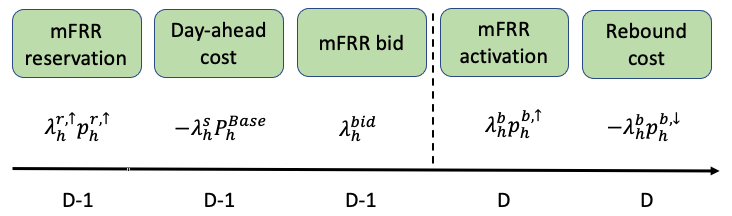
\includegraphics[width=0.99\textwidth]{figures/timeline_mfrr.png}
    \caption{Timeline of cost components in (\ref{eq:mFRRObjective}). }
    \label{fig:timeline_mfrr}
\end{figure}

\subsection{Load shifting}

\section{Grey-box modelling}

\textcolor{red}{Most - if not all - of this goes to appendix}
\subsection{Prediction error method vs simulation errors}


\section{Thermostatically controlled loads}

TCLs are characterized by being controlled such that the temperature is kept at a specified setpoint. Examples includes heat pumps, freezers, air condition units, ovens, etc. They are widely believed to constitute an important part of demand-side flexibility due to the inherent thermal inertia of such temperature-driven systems.

In this paper, we focus on freezers, which are a common type of TCL. Specifically, we focus on a single freezer display in a Danish supermarket. Freezers are characterized by a large thermal inertia due to the frozen food, which makes them suitable for flexibility. On the other hand, the there is a risk of food degradation when utilizing flexibility. Therefore, it is important to model the temperature dynamics in the freezer for a realistic estimation of its flexibility.

The rest of the section is organized as follows. First, we visualize the most important measurements from a real supermarket freezer. Second, we introduce a second-order model that characterizes the supermarket freezer. Third, we validate the second-order model and show how it can be used to simulate a demand response from a freezer.

\subsection{Visualization of freezer measurements}

\begin{figure}[H]
    \centering
    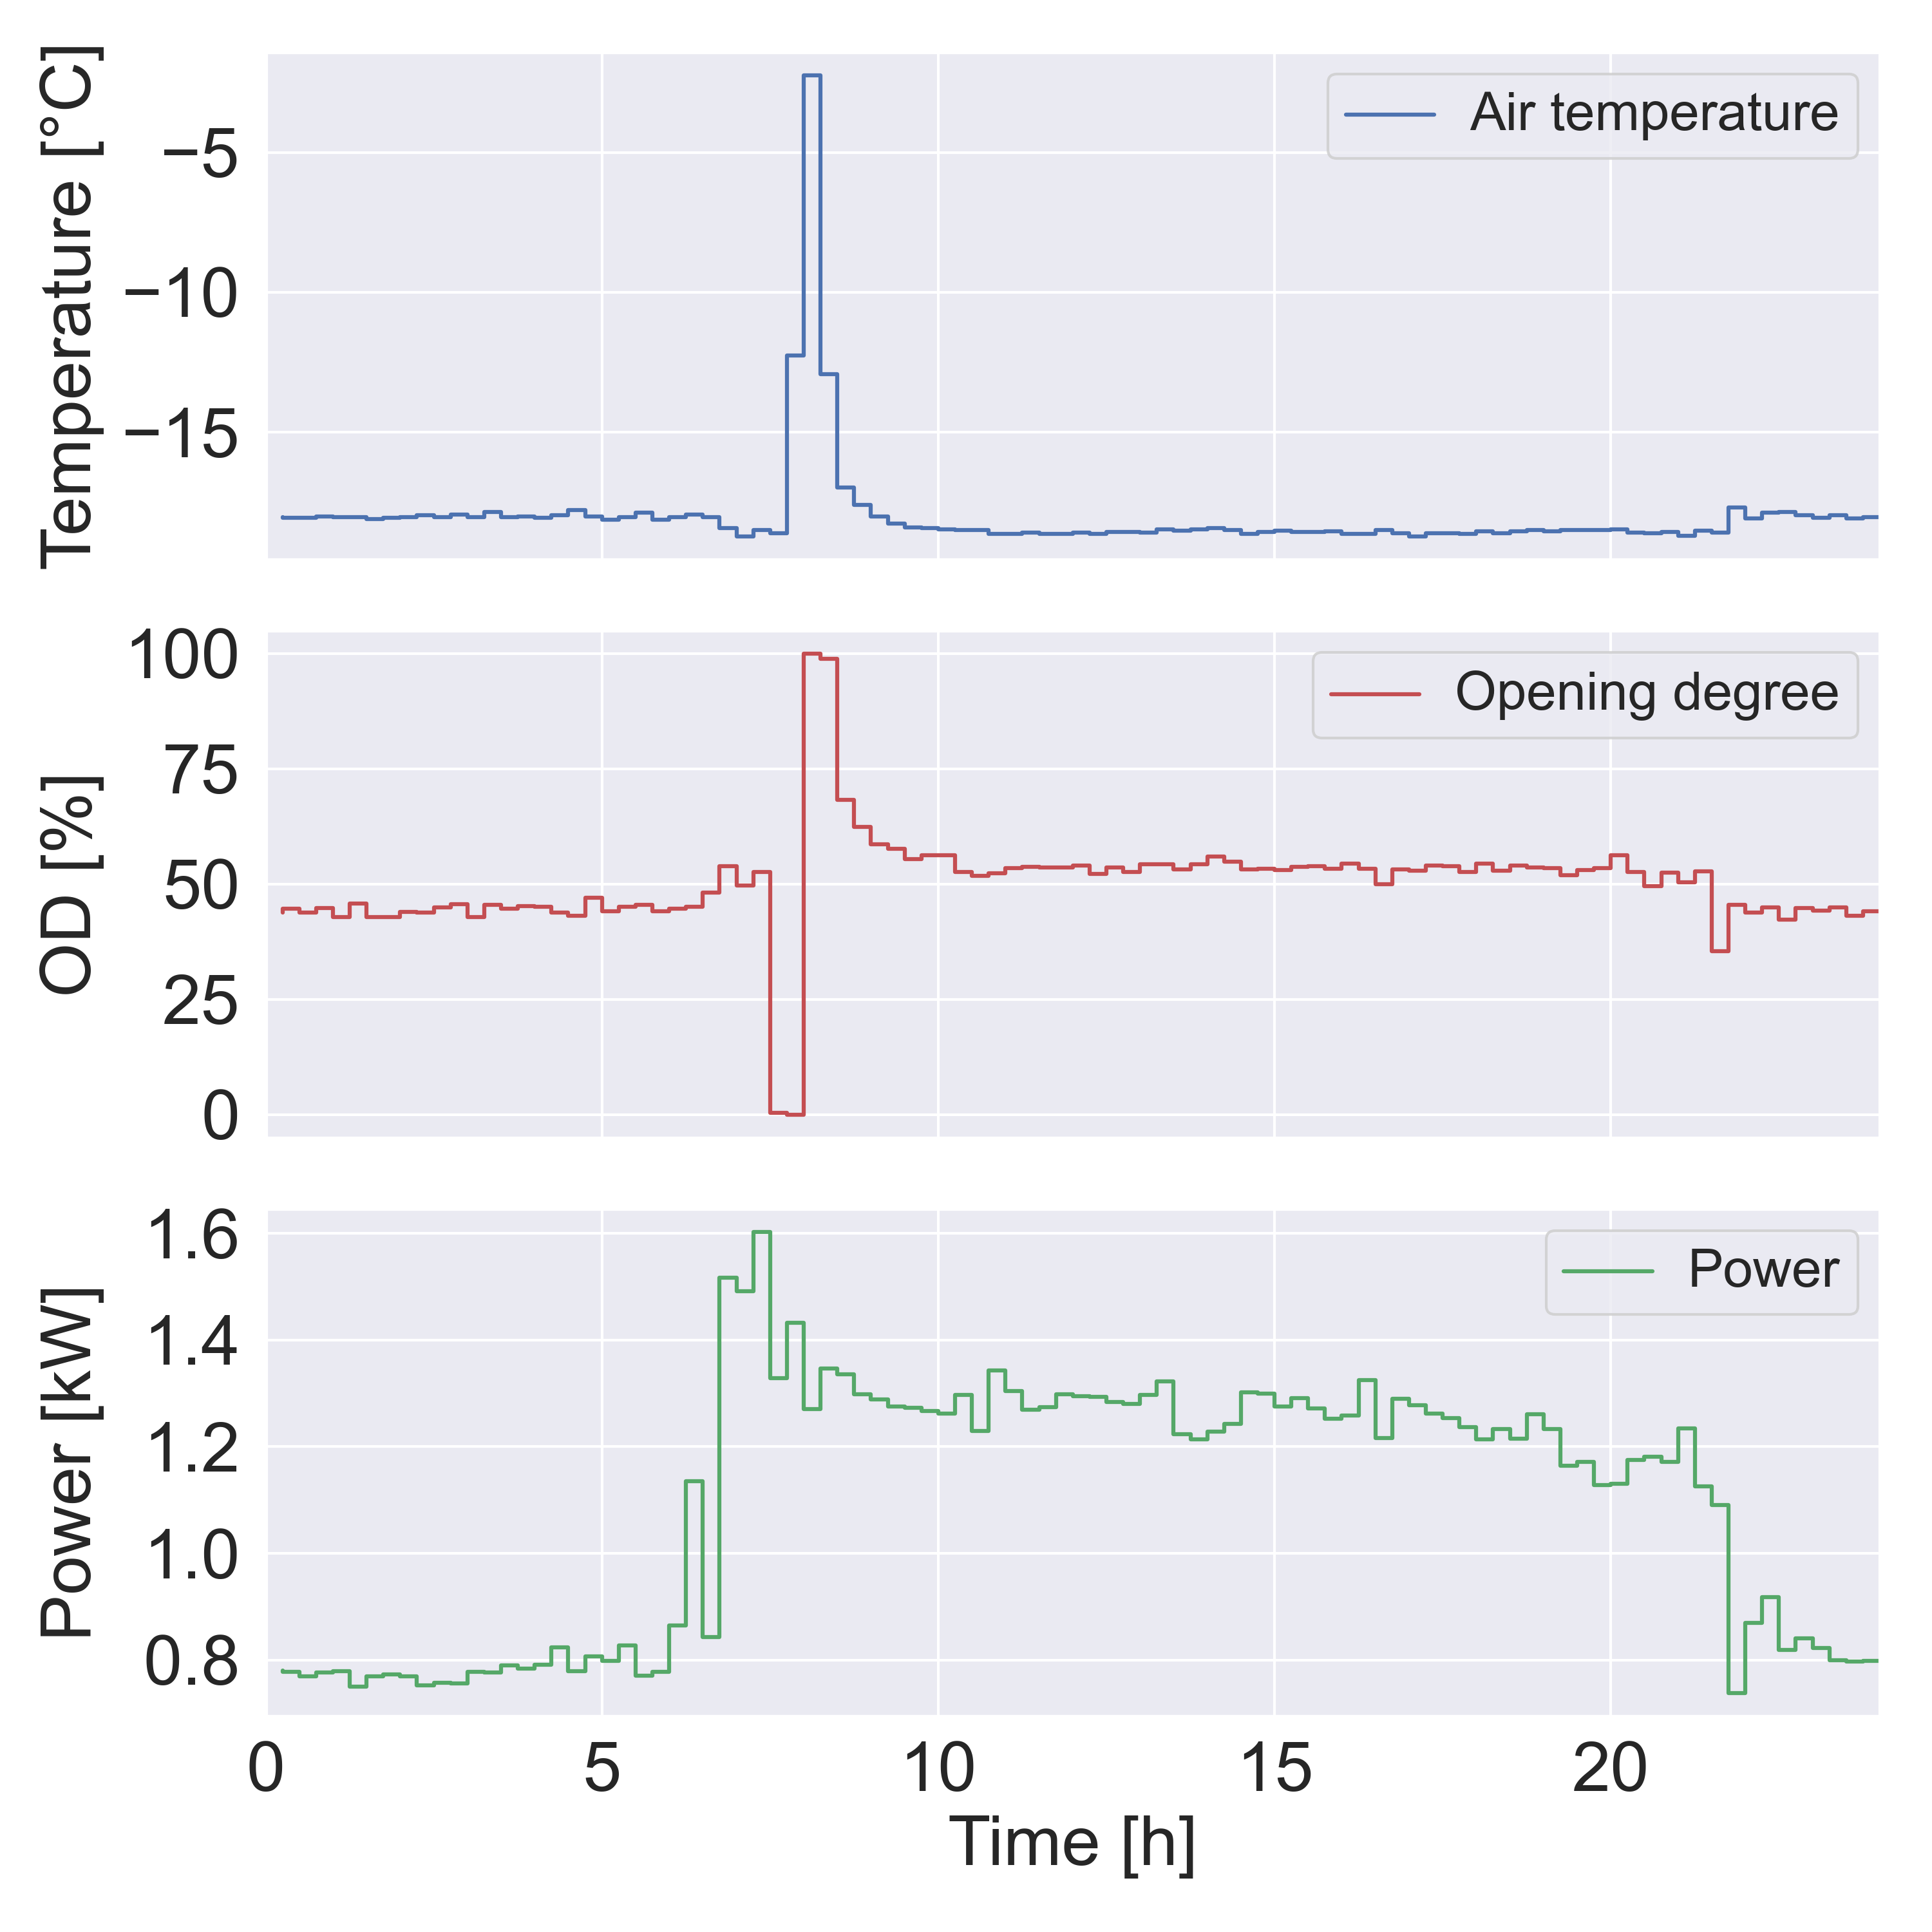
\includegraphics[width=0.99\textwidth]{figures/tmp_od_Pt.png}
    \caption{\textbf{Top}: yearly average temperature of a single freezer in a supermarket. \textbf{Middle}: opening degree of the freezer expansion valve. \textbf{Bottom}: power of the compressors feeding all the freezers (scaled to only include all freezers in the supermarket).}
    \label{fig:chunk}
\end{figure}

\subsection{Thermal modelling of freezer}

In Appendix \ref{appendix:A}, it is described how a simple TCL model can be made. We extend it to a second-order model that accounts for the thermal mass of the food, which essentially provides the flexibility in freezers:

\begin{subequations}\label{eq:2ndFreezer}
    \begin{align}
        \frac{dT^f(t)}{dt} & = \frac{1}{C^f}\left(\frac{1}{R^{cf}} (T^c(t) - T^f(t)) \right)                                                                                  \\
        \frac{dT^c(t)}{dt} & = \frac{1}{C^c}\Bigl(\frac{1}{R^{cf}} (T^f(t) - T^c(t)) + \frac{1}{R^{ci}(t)} (T^i(t) - T^c(t))                                         - \notag \\ & \mspace{50mu} \eta \cdot OD(t) P(t) \Bigr) + \epsilon \mathbbm{1}^{df}
    \end{align}
\end{subequations}

In state-space form, it is:

\begin{subequations}\label{eq:2ndFreezerStateSpace}
    \begin{align}
        T^{f}_{t+1} & = T^{f}_{t} + dt \cdot \frac{1}{C^f}\left(\frac{1}{R^{cf}} (T^{c}_{t} - T^{f}_{t}) \right)                                                                               \\
        T^{c}_{t+1} & = T^{c}_t + dt \cdot \frac{1}{C^c}\Bigl(\frac{1}{R^{cf}} (T^{f}_t - T^{c}_t) + \frac{1}{R^{ci}_{t}} (T^{i}_t - T^{c}_t)                                         - \notag \\ & \mspace{50mu} \eta \cdot OD_t P_t \Bigr) + \epsilon \mathbbm{1}^{df}
    \end{align}
\end{subequations}


Here, $T^c$ is the air temperature in the freezer, and $T^f$ is the food temperature which is a latent, unobserved state. It is essentially a low-pass filter of the air temperature in the freezer with time constant $\tau = C^f R^{cf}$. $C^f$ and $C^c$ are the thermal capacitance of the food and air in the freezer, respectively. $R^{cf}$ and $R^{ci}$ are the thermal resistance between food and air, and air and indoor temperature, respectively. Furthermore, $\epsilon$ represents the temperature change when defrosting and $\mathbbm{1}^{df}$ is an indicator for when defrosting happens. $R^{ci}$ is time-varying to capture the differences between opening- and closing hours. The opening degree, $OD_t$, and power $P_t$, are exogenous inputs.

\subsection{Validation and simulation}

\begin{figure}[!ht]
    \centering
    \begin{subfigure}[b]{.49\textwidth}
        \centering
        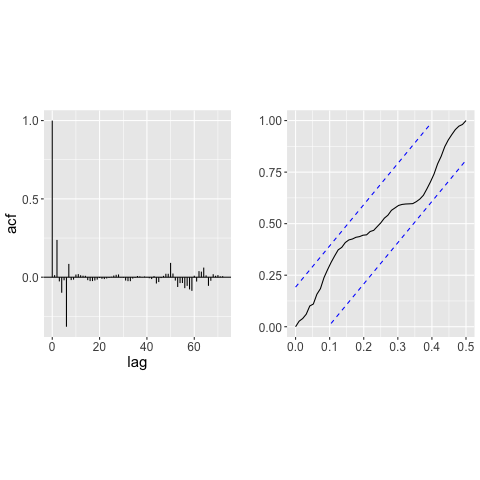
\includegraphics[width=0.89\textwidth]{figures/2ndFreezerModelValidation.png}
        \caption{Validation of the state-space model in (\ref{eq:2ndFreezerStateSpace}). Left: auto-correlation function of the model residuals. Right: cumulated periodogram of the residuals.}
        \label{fig:2ndFreezerModelValidation}
    \end{subfigure}
    \hfill
    \begin{subfigure}[b]{.49\textwidth}
        \centering
        \begin{tabular}[b]{|l|l|l|}
            \hline
            Parameter       & Value & Unit            \\ \hhline{|=|=|=|}
            $C^f$           & 5.50  & kWh/$^{\circ}$C \\
            $C^c$           & 0.13  & kWh/$^{\circ}$C \\
            $R^{cf}$        & 4.91  & $^{\circ}$C/kW  \\
            $R^{ci, day}$   & 25.6  & $^{\circ}$C/kW  \\
            $R^{ci, night}$ & 46.5  & $^{\circ}$C/kW  \\
            $\eta$          & 2.38  &                 \\
            $\epsilon$      & 6.477 & $^{\circ}$C/h   \\ \hline
        \end{tabular}
        \newline
        \newline
        \newline
        \caption{Parameter estimates of eq. (\ref{eq:2ndFreezerStateSpace}). \newline \newline}%
        \label{tab:2ndFreezerParam}
    \end{subfigure}
\end{figure}


\begin{figure}[H]
    \centering
    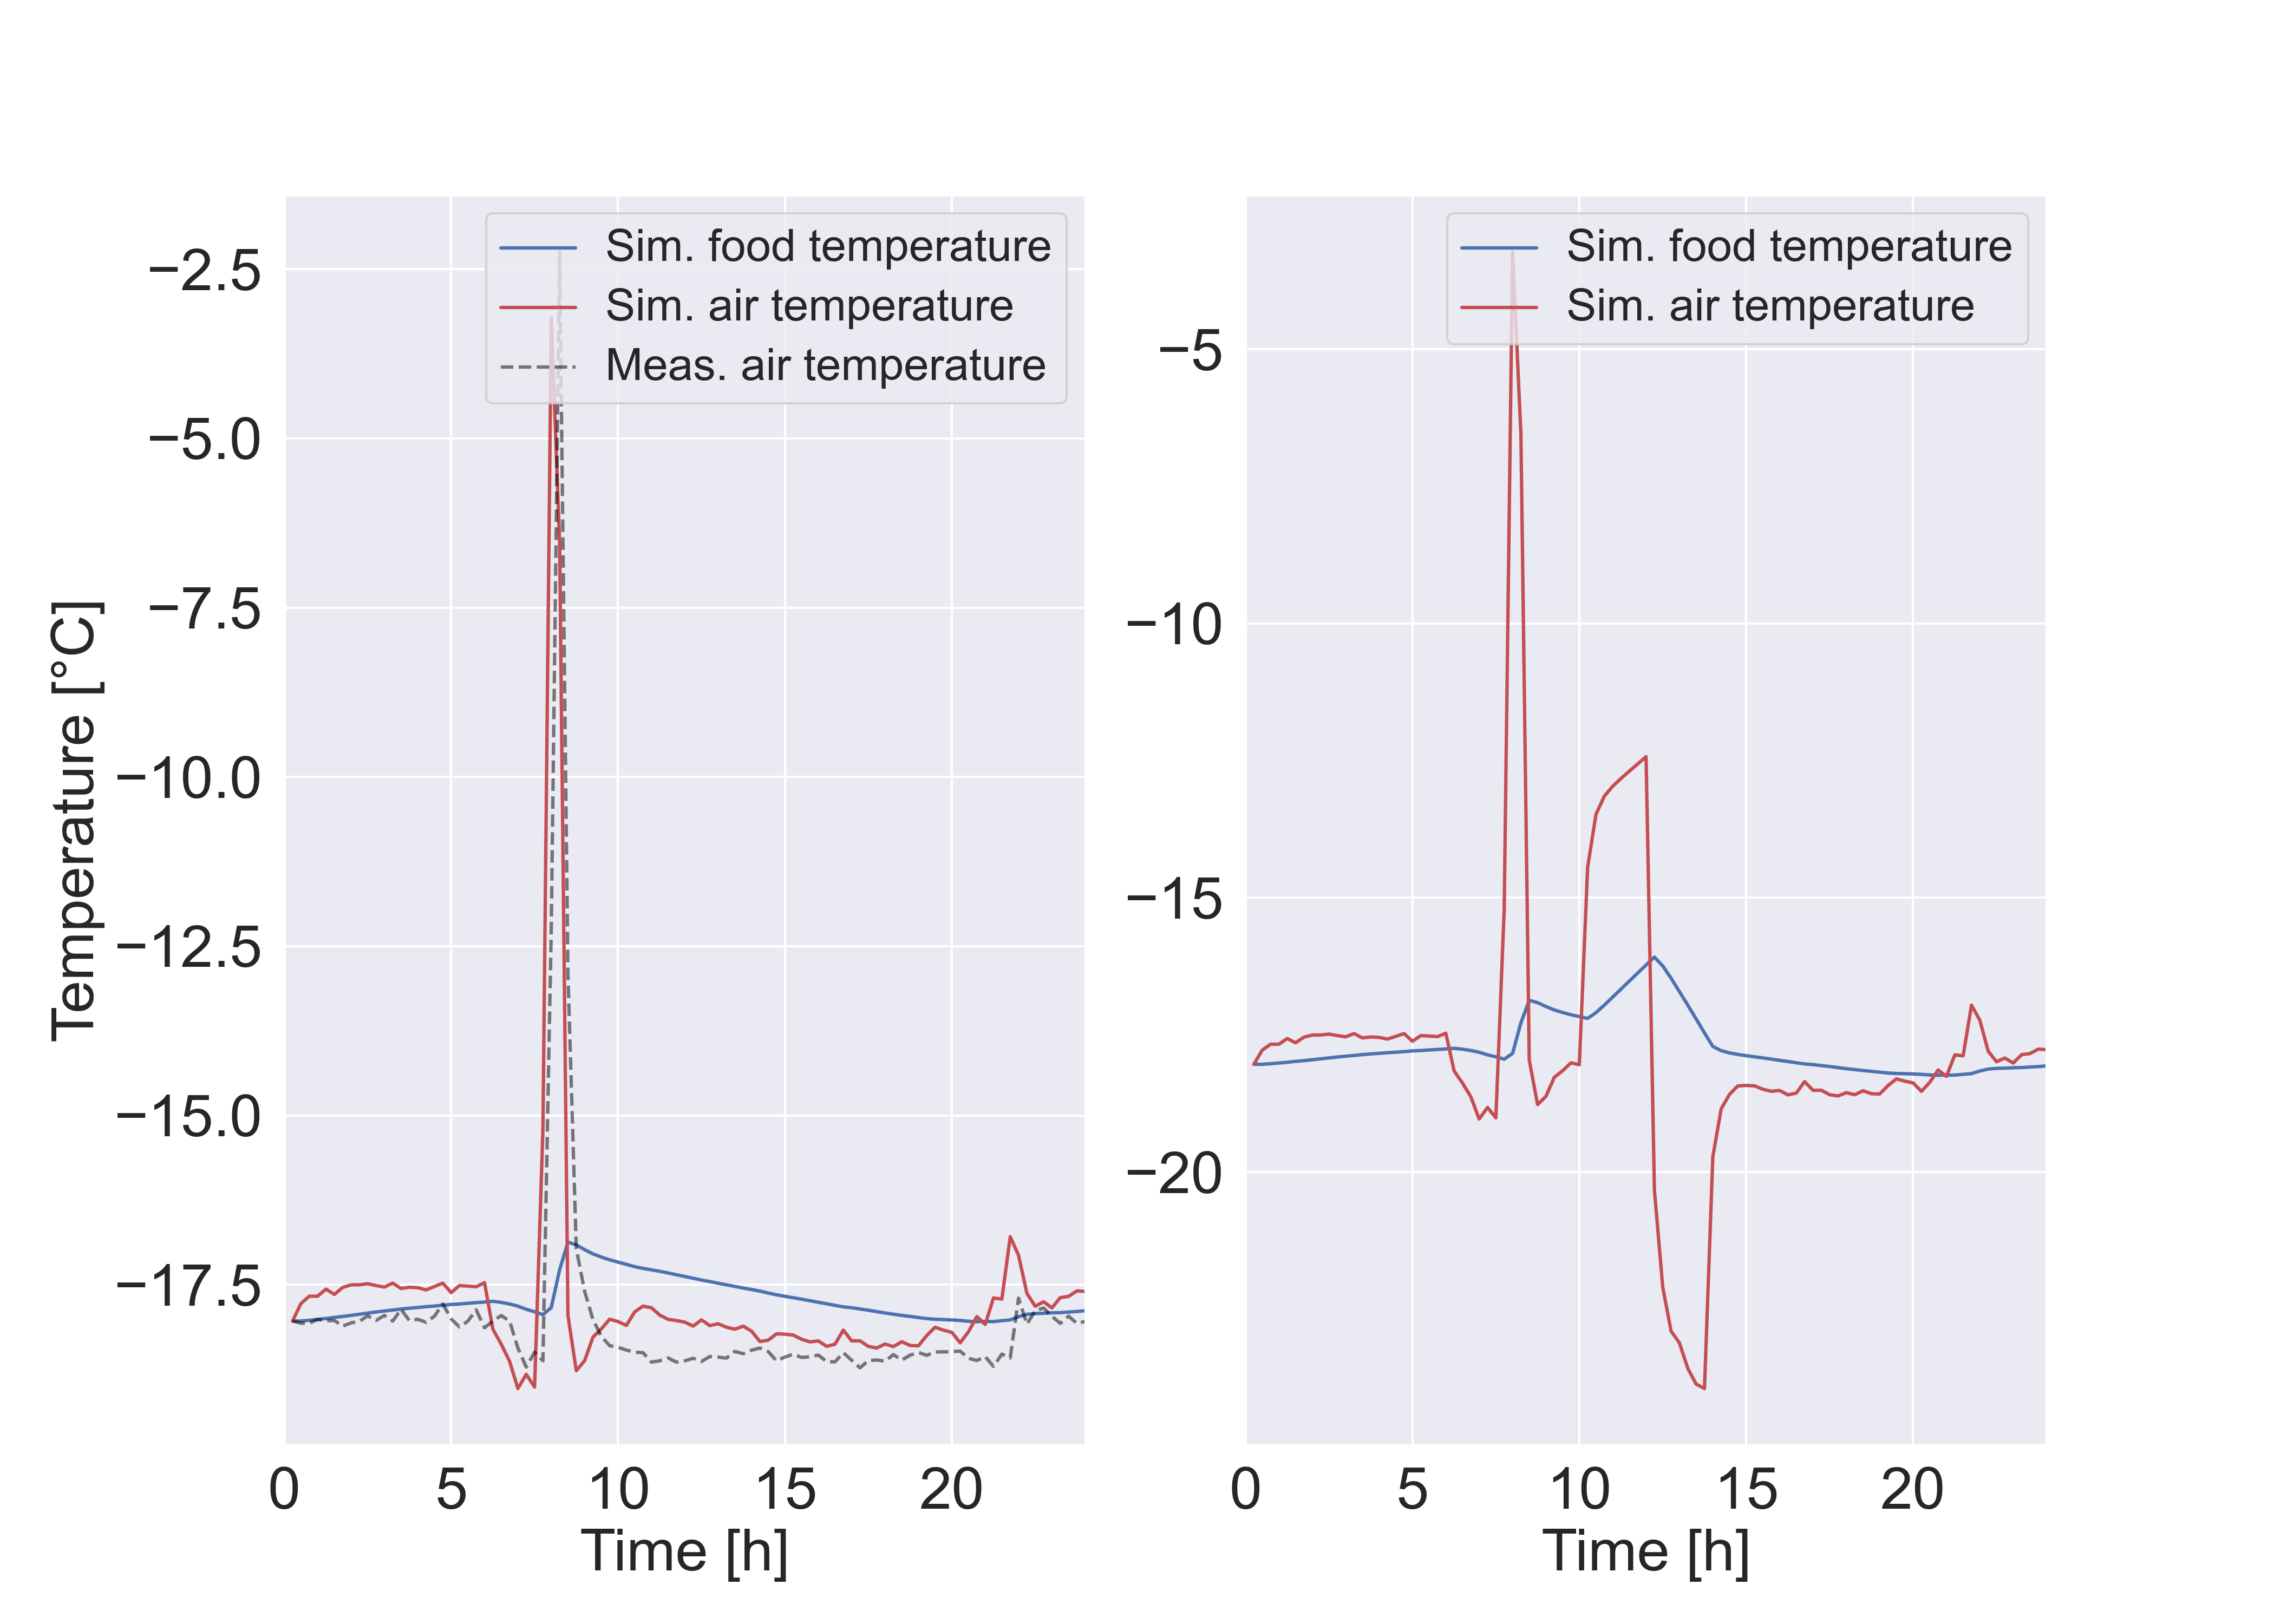
\includegraphics[width=0.99\textwidth]{figures/2ndFreezerModelSimulation.png}
    \caption{ \textbf{Left}: Simulation of (\ref{eq:2ndFreezerStateSpace}) using the parameters in Table \ref{tab:2ndFreezerParam} \textbf{Right}: Simulation where power is turned off for two hours with a subsequent rebound at the nominal power until the food temperature is back to its normal value.}
    \label{fig:2ndFreezerModelSimulation}
\end{figure}

\section{Optimization model}

\subsection{Objective function}

\subsection{Scenario generation}

\subsection{Decomposition}

Write about ADMM to solve the optimization problem.


\section{Results}

\subsection{ADMM}

\begin{figure}[H]
    \centering
    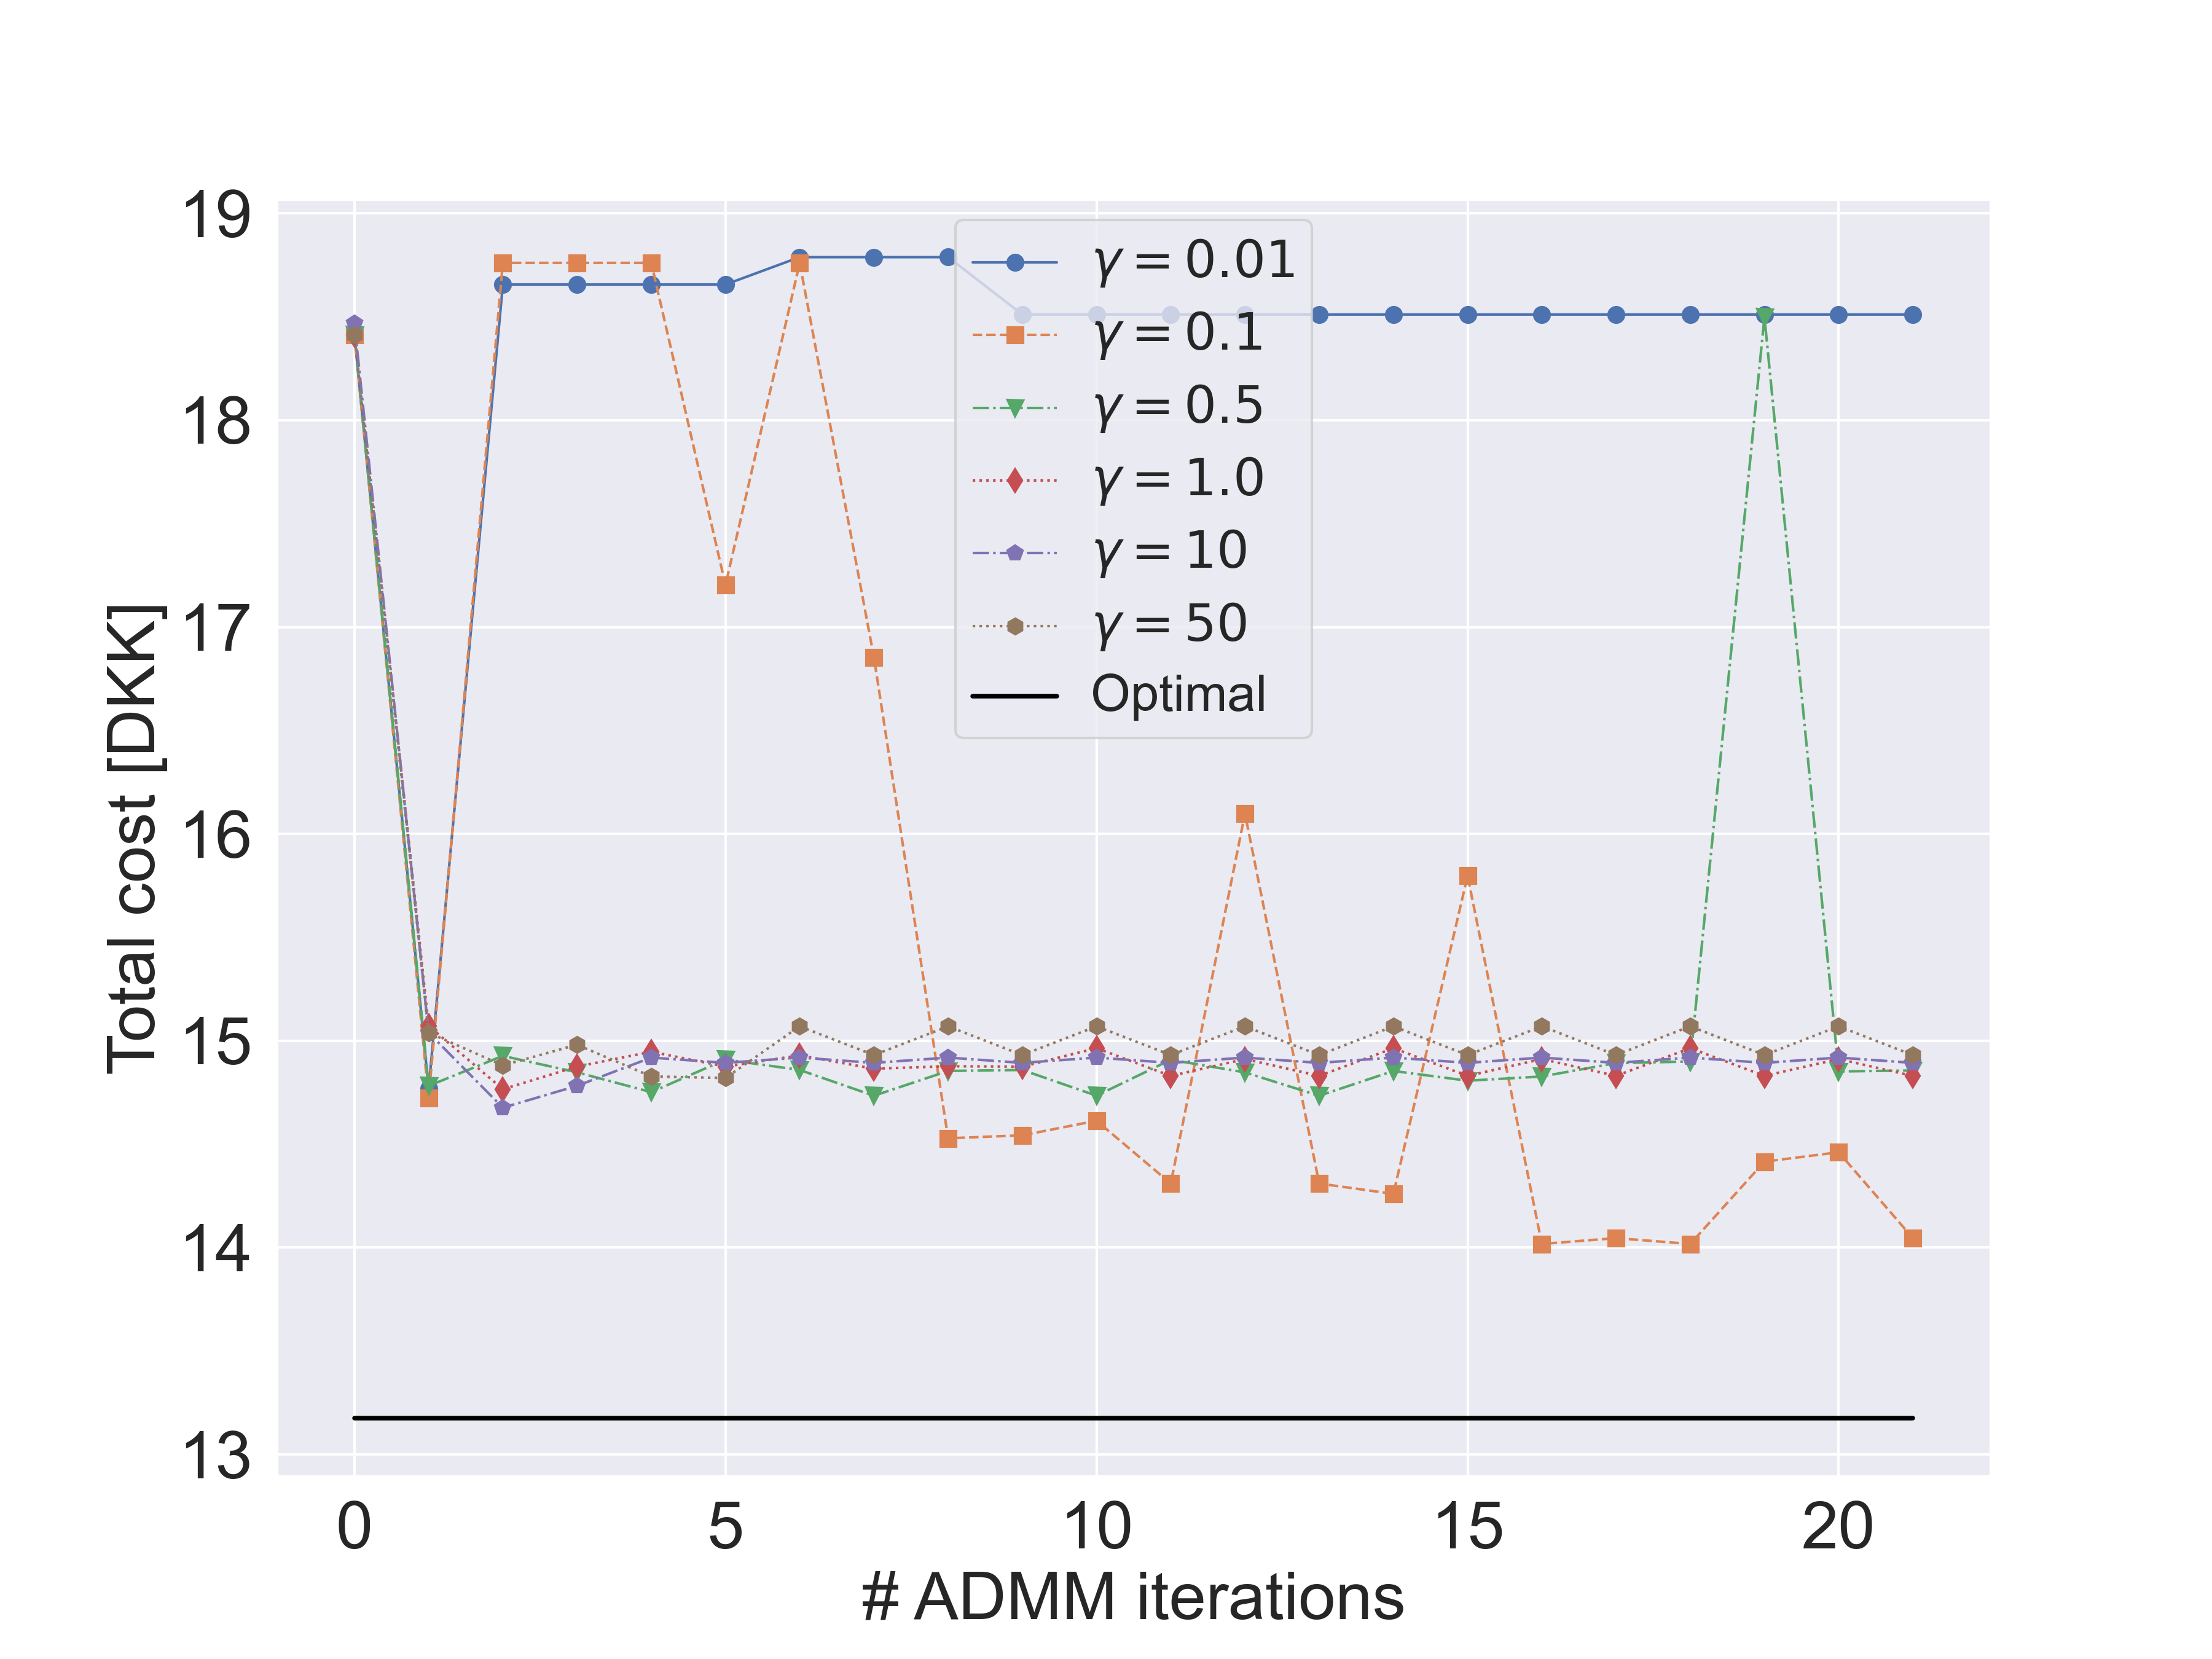
\includegraphics[width=0.99\textwidth]{figures/admm_vs_normal_solution.png}
    \caption{ADMM solution versus the optimal solution for five scenarios.}
    \label{fig:admm_vs_normal_solution}
\end{figure}

\begin{figure}[H]
    \centering
    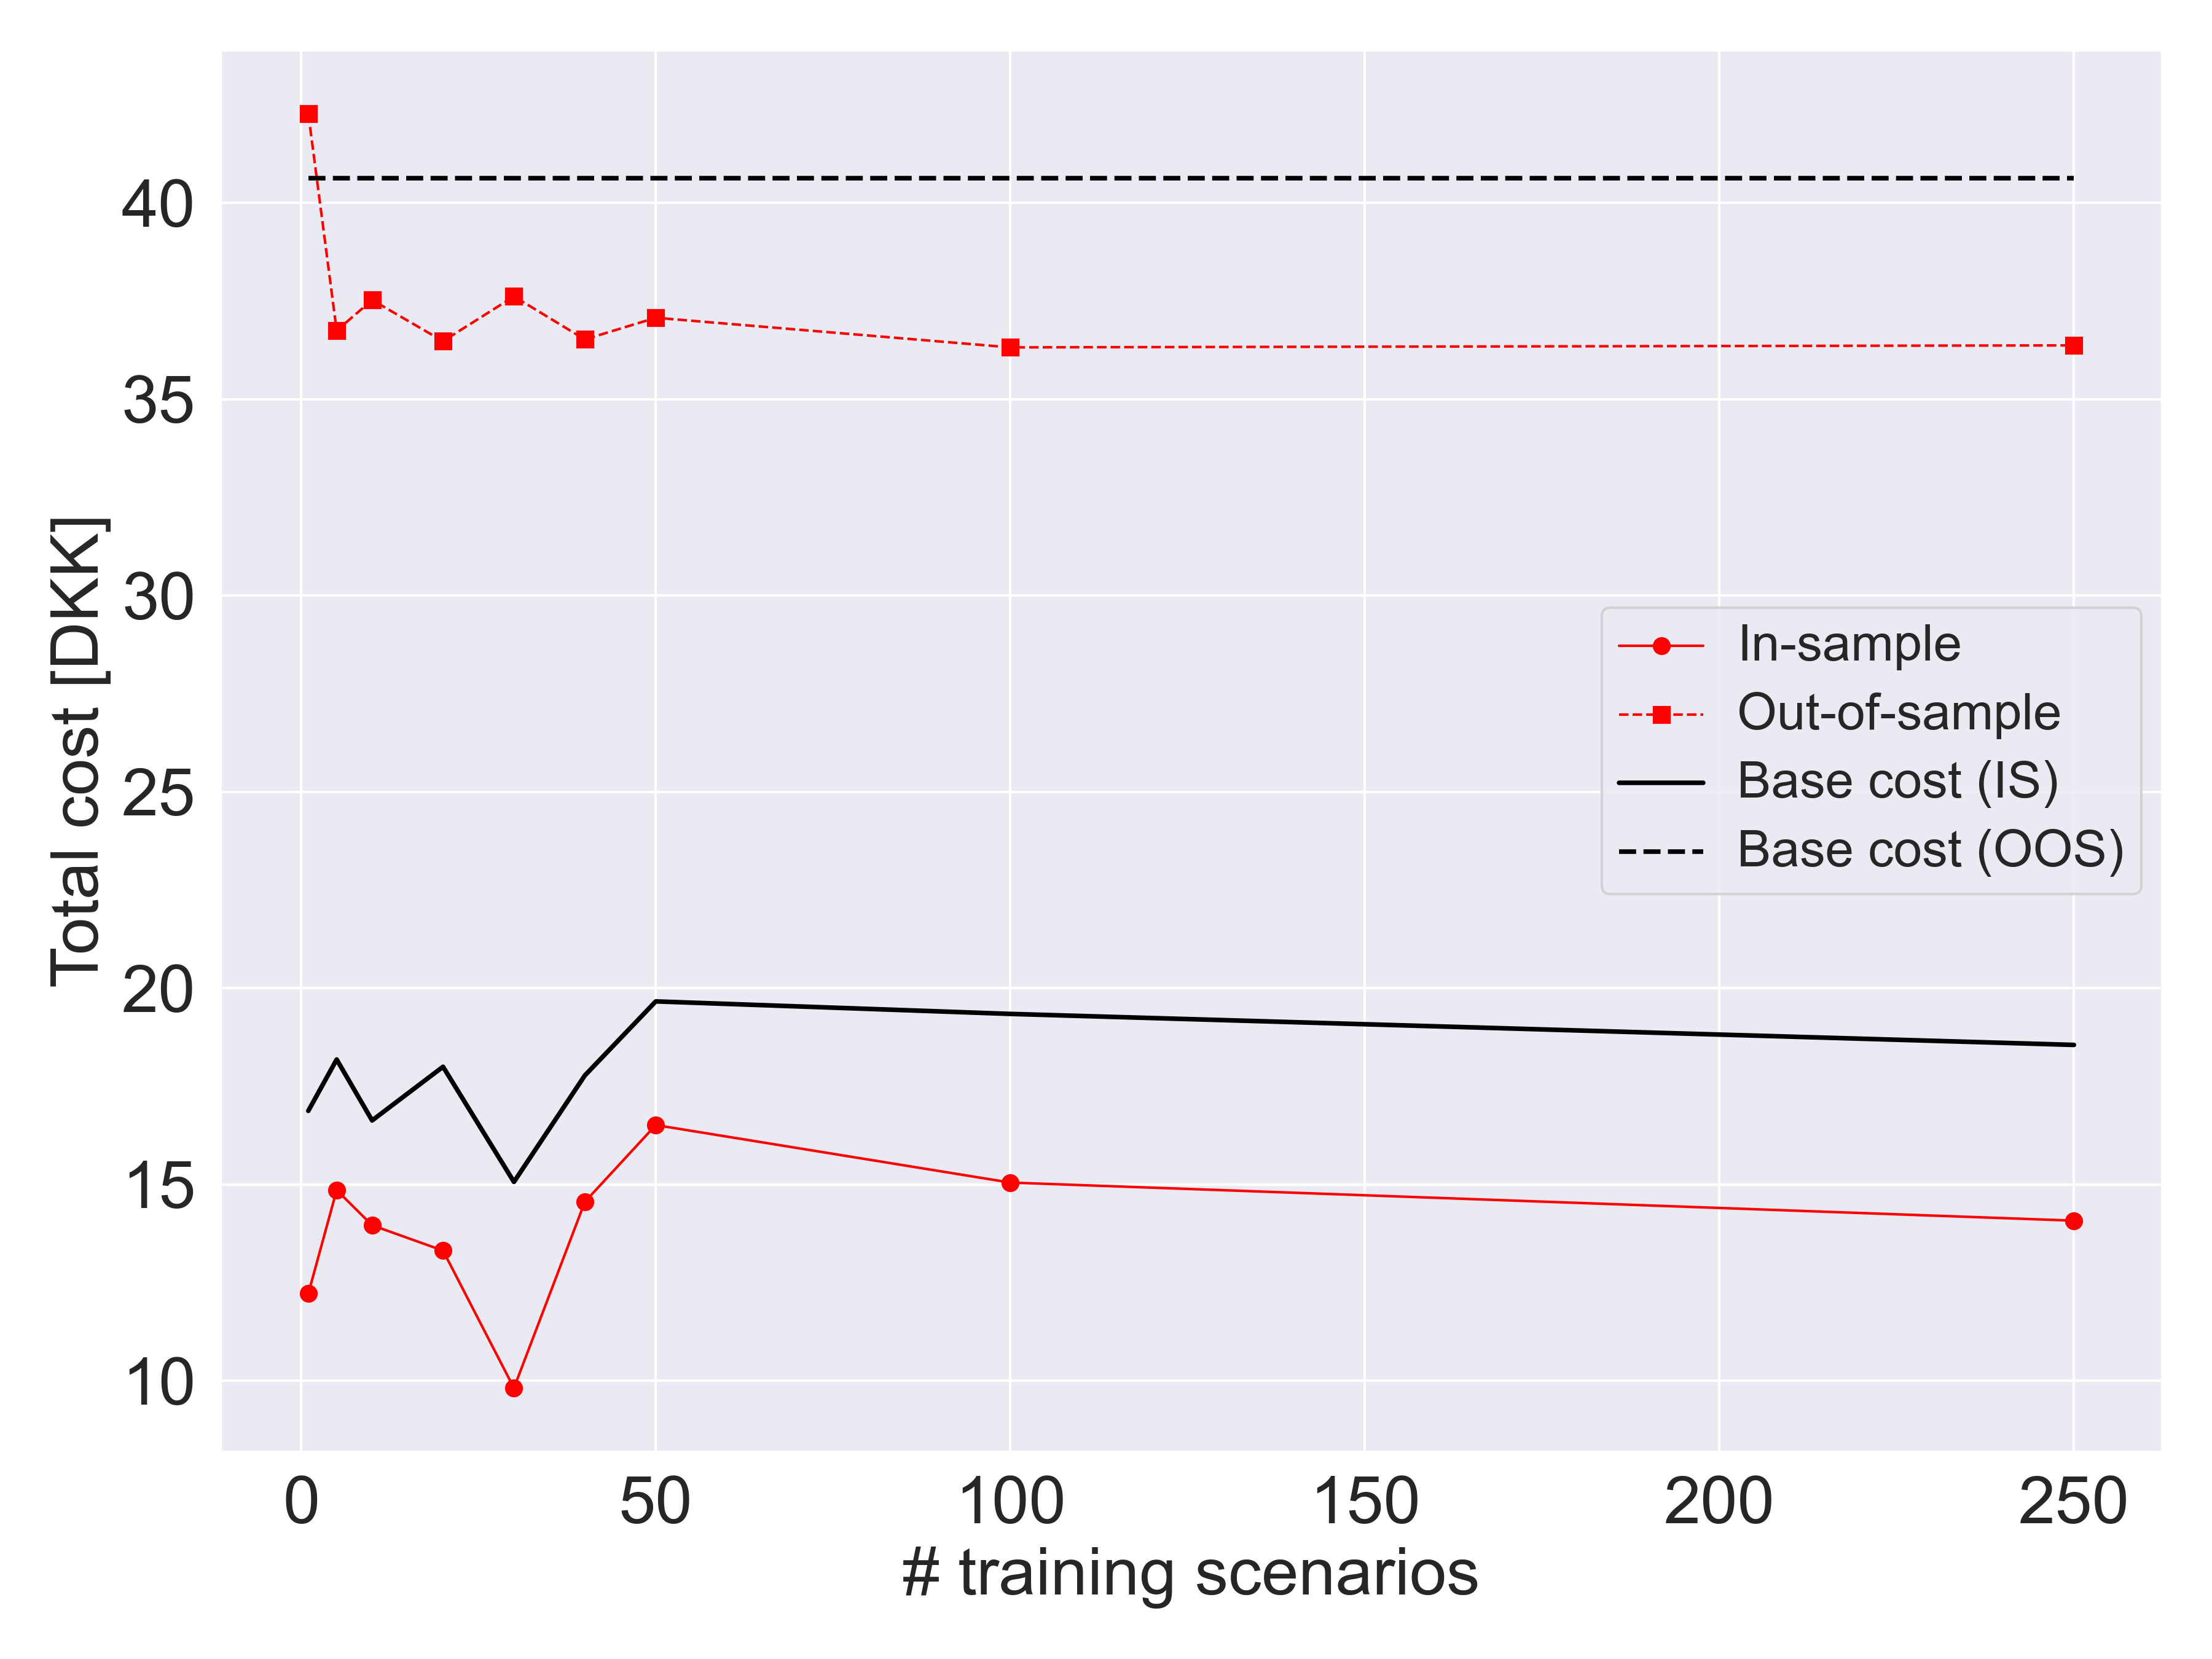
\includegraphics[width=0.99\textwidth]{figures/admm_nb_scenarios_effect.png}
    \caption{Effect of number of in-sample scenarios on out-of-sample performance for ADMM. Both are compared to the baseline costs of the freezer.}
    \label{fig:admm_nb_scenarios_effect}
\end{figure}

\subsection{Lookback}

TODO: create plot of effect of lookback parameter.

\subsection{Load shifting vs mFRR}

\begin{figure}[H]
    \centering
    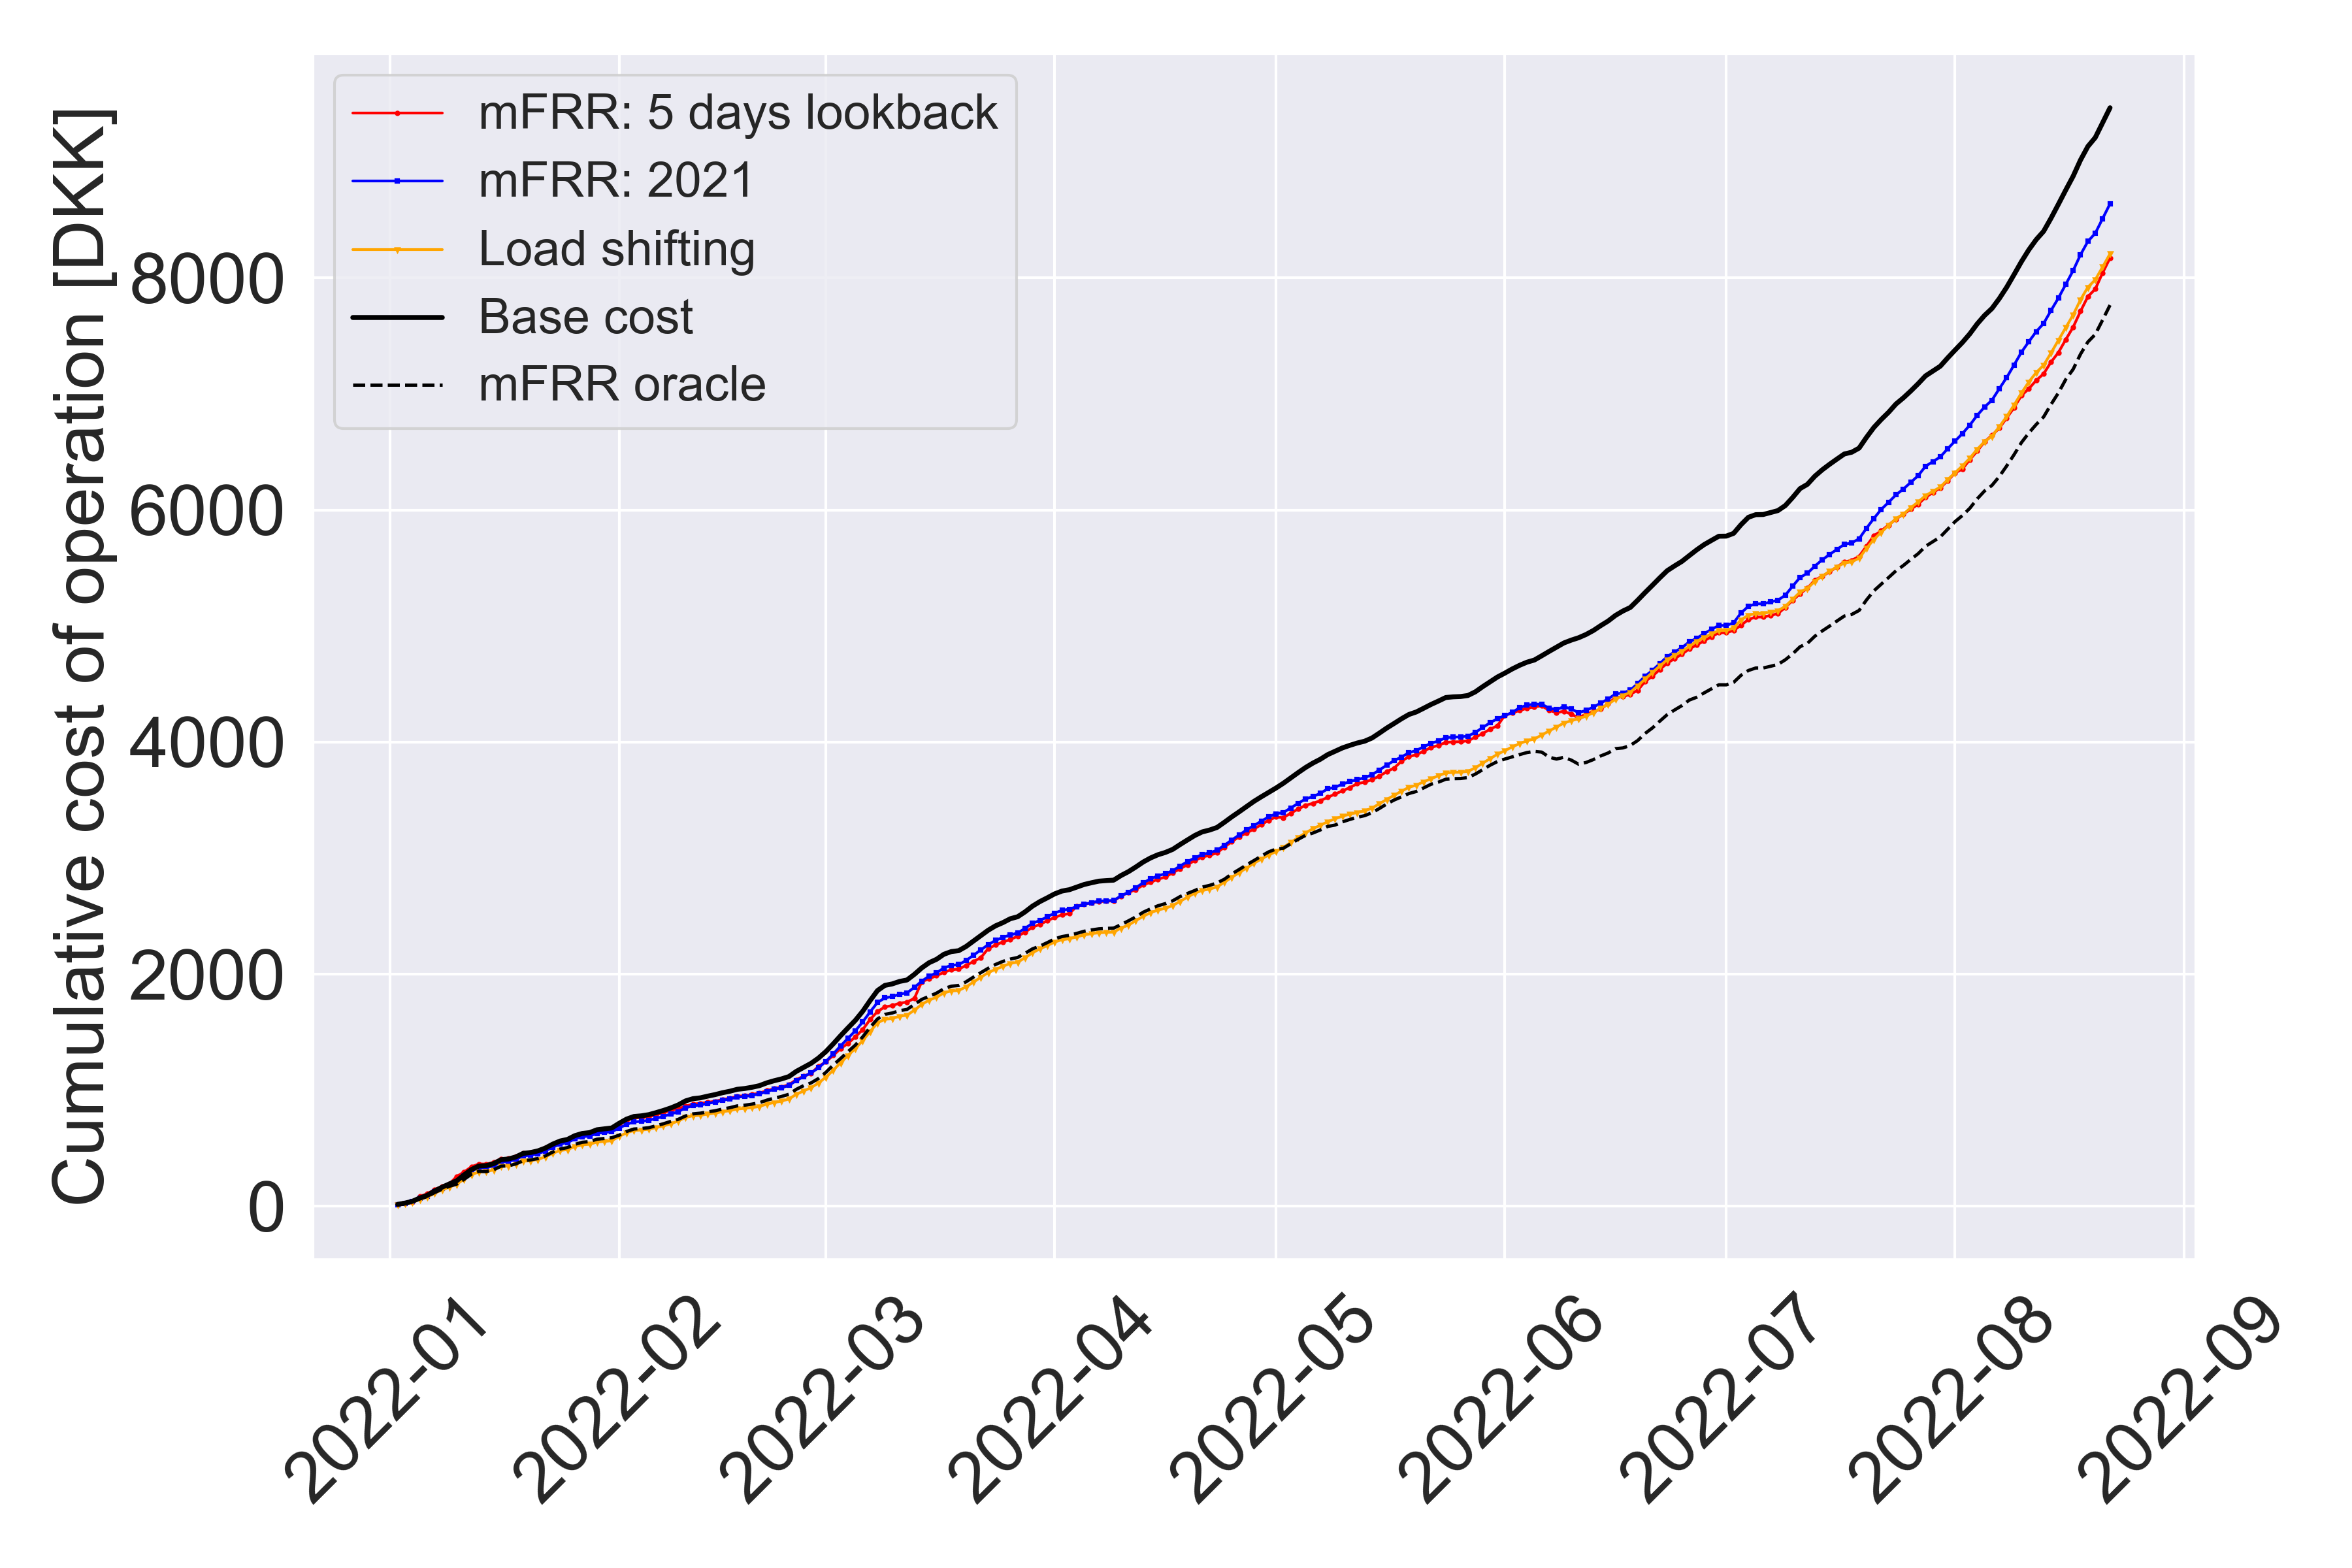
\includegraphics[width=0.99\textwidth]{figures/cumulative_cost_comparison.png}
    \caption{Out-of-sample cumulative costs for load shifting and mFRR using ADMM with 50 scenarios and a lookback of 5 scenarios.}
    \label{fig:cumulative_cost_comparison}
\end{figure}

\begin{figure}[H]
    \centering
    \makebox[\linewidth][c]{%
        \begin{subfigure}[t]{.65\textwidth}
            \centering
            \captionsetup{width=.90\linewidth}
            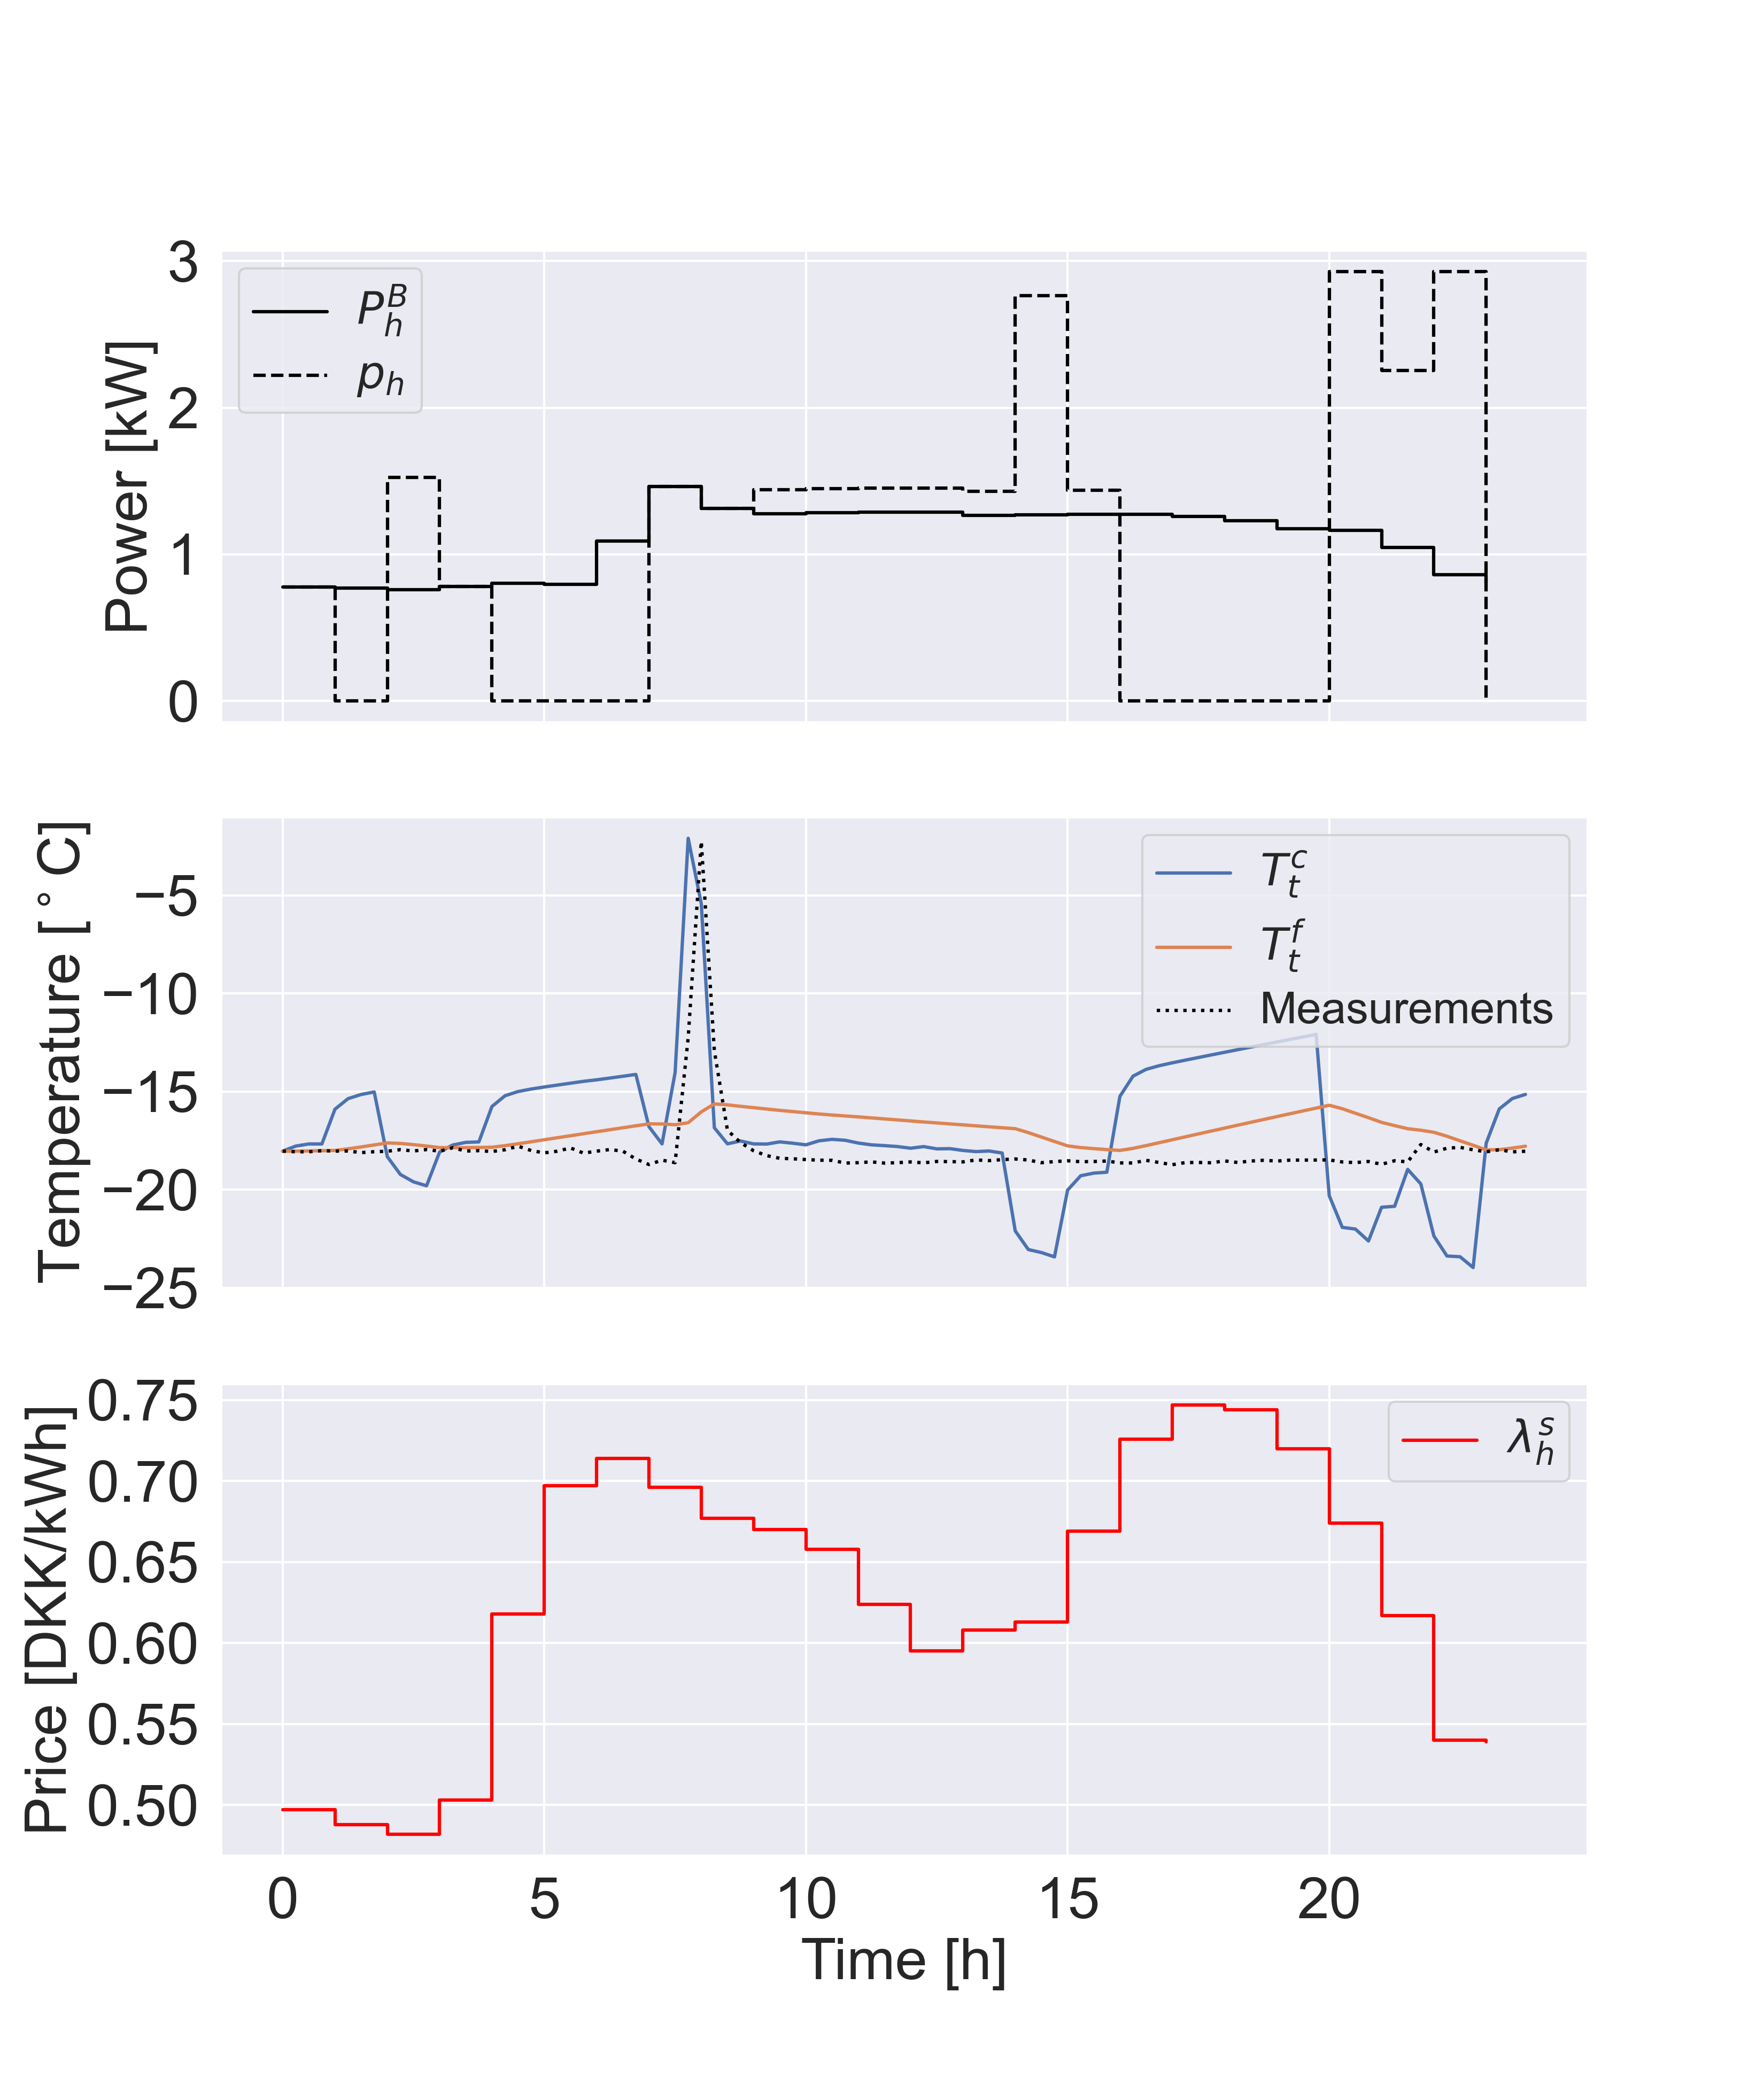
\includegraphics[width=.95\linewidth]{figures/spot_single_case.png}
            \caption{\textbf{Top}: Power profile when load shifting and baseline power of freezer. \textbf{Middle}: Air and food temperature dynamics. \textbf{Bottom}: Spot price in scenario.}
            \label{fig:spot_single_case}
        \end{subfigure}%
        \hfill
        \begin{subfigure}[t]{.65\textwidth}
            \centering
            \captionsetup{width=.90\linewidth}
            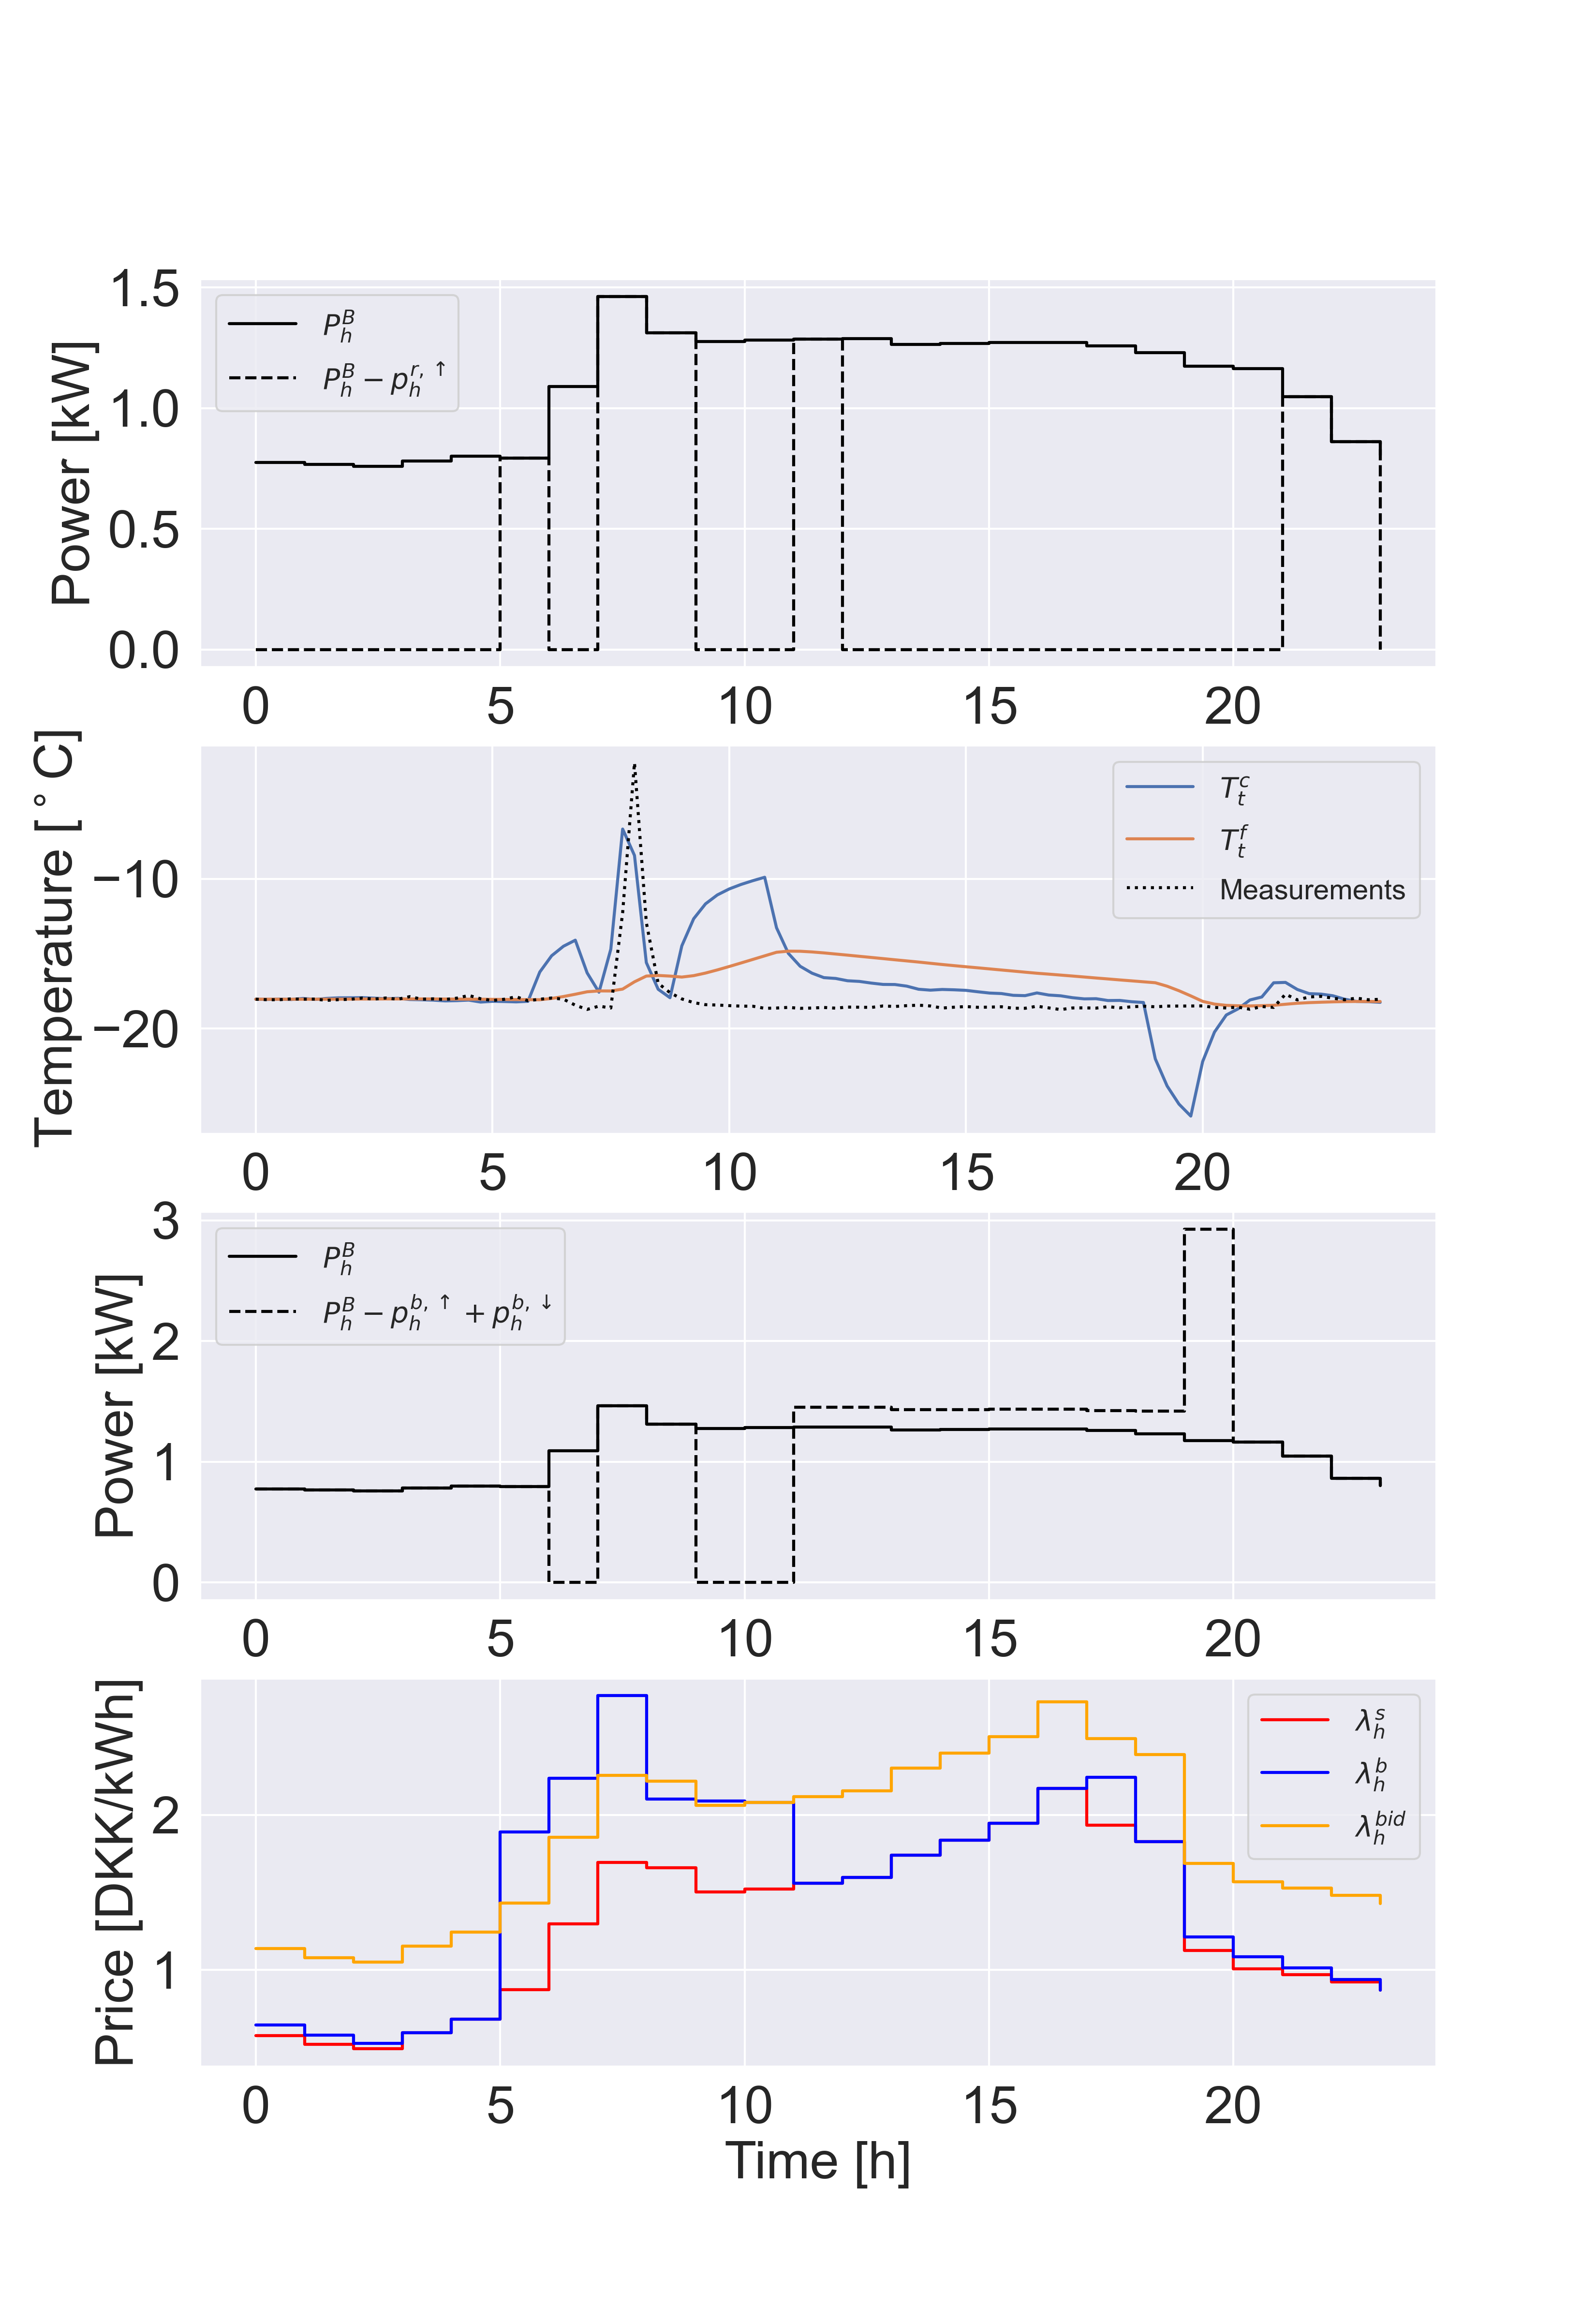
\includegraphics[width=.95\linewidth]{figures/mFRR_single_case.png}
            \caption{\textbf{Top}: Reservation capacities and baseline power of freezer. \textbf{Upper middle}: Air and food temperature dynamics. \textbf{Lower Middle}: mFRR activations in this scenarios, i.e., when $\lambda_{h}^{bid} \leq \lambda_{h}^{b}$ and $\lambda_{h}^{b} > \lambda_{h}^{s}$ and $p^{r,\uparrow}_{h} > 0$. \textbf{Bottom}: Spot price, balancing price, and bid in scenario.}
            \label{fig:mFRR_single_case}
        \end{subfigure}%
    }
    \caption{Comparison between load shifting and mFRR in one scenario in-sample. \textbf{Left}: Load shifting. \textbf{Right}: mFRR.}
    \label{fig:load_shift_case_vs_mFRR_case}
\end{figure}

\begin{table}[H]
    \caption{Out-of-sample costs of freezer in [DKK/day] for mFRR with five days lookback, load shifting, and mFRR trained with 50 in-sample scenarios using ADMM.}
    \label{tab:cases_compared}
    \centering
    \begin{tabular}{lccc}
        \toprule
        Name                 & mFRR w. lookback & Load shifting & mFRR w. 2021 \\
        \midrule
        Base cost today      & 40.628           & 40.628        & 40.628       \\
        Total cost           & 35.918           & 34.994        & 36.514       \\
        Expected energy cost & 40.628           & 34.994        & 40.628       \\
        Rebound cost         & 0.858            & 92.869        & 0.911        \\
        Reserve payment      & 3.216            & 0.0           & 3.381        \\
        Act payment          & 8.092            & 0.0           & 2.161        \\
        Penalty cost         & 5.741            & 0.0           & 0.516        \\
        Scenarios            & -5               & 1             & 50           \\
        Admm                 & False            & False         & True         \\
        \% savings           & 11.6             & 13.9          & 10.1         \\
        \bottomrule
    \end{tabular}
\end{table}

\section{Discussion}


\vspace{-2mm}
\section{Conclusion}\label{sec:conclusion}
%
We investigated how a supermarket freezer can provide flexibility for mFRR and load shifting in Denmark, and explored which one provides a greater monetary incentive for a flexible load. To this end, we used actual data  from a Danish supermarket. This was done by developing a second-order grey-box model of the temperature dynamics in the freezer with the food temperature as a latent state. In the state-space form, the model was directly incorporated as constraints into a two-stage stochastic MILP problem, whose objective is to maximize the monetary value from the freezer's flexibility. Two scenario generation strategies were implemented: one with a five-day lookback strategy on the spot and balancing market prices in DK2, and the other one  based on price data for those markets in 2021. For mFRR, we used a linear policy, and then linearized the conditions for activation via the McCormick relaxation method. For computational ease, we used an ADMM-based scenario decomposition technique.  An out-of-sample evaluation was done on unseen 2022 price data. We observed that load shifting is more profitable, but has a greater impact on the air and food temperatures in the freezer as opposed to mFRR that depends on the system state and bid price for activation.

We made a set of simplifications and assumptions, whose impacts need to be explored for the future work. The revenue share of BRP and aggregator was not considered. This may change our finding that load shifting is more financially appealing to a flexible load. As mentioned earlier, a single freezer or supermarket must be part of a larger portfolio through an aggregator in order to participate in the mFRR market. Such an aggregated portfolio has some issues that are neglected here, such as the baseline estimation for verification of the demand response, allocation of profits within the portfolio, and an accurate capacity estimation of the whole portfolio that bids in the mFRR market. Furthermore, the European mFRR markets will change from a 60-minute resolution to a 15-minute market in the next few years \cite{MARI}. This makes it more feasible for TCLs to participate in the mFRR market, given their sensitivity to large temperature deviations, and the fact that TCLs can get a passive income when there is no up-regulation need in the power grid.

Test that I can refer to \gls{OOS} and \gls{IS}.

{\appendices

\section*{Appendix: Final model formulation}\label{appendix:A}
% \addcontentsline{toc}{section}{Appendices}
% \renewcommand{\thesubsection}{\Alph{subsection}}
% \subsection{Appendix}\label{appendix:A}

%\subsection{Final model formulation}\label{sec:final_model}

% Describe objective function for mFRR and load shifting.

% The set, $\Psi$, then contains all the optimization variables:

% \begin{align}\label{set:OptVariables}
%     \Psi = \{p_{h,\omega}, p^{r, \uparrow}_{h}, & s_{h,\omega}, p^{b, \uparrow}_{h,\omega}, p^{b, \downarrow}_{h,\omega}, u^{\uparrow}_{h,\omega}, y^{\uparrow}_{h,\omega}, z^{\uparrow}_{h,\omega}, u^{\downarrow}_{h,\omega}, y^{\downarrow}_{h,\omega}, z^{\downarrow}_{h,\omega}, \notag \\ & T^{f}_{\omega, t}, T^{c}_{\omega, t}, T^{f,B}_{t}, T^{c, B}_{t}, \lambda_{h}^{bid}, \phi_{h,\omega}, g_{h,\omega}, \Delta \}
% \end{align}


\begingroup
\allowdisplaybreaks

The final optimization model is a two-stage stochastic MILP and is described in full detail in (\ref{FinalModel}) with subsequent explanations.
% First, the objective function is presented. Then all auxillary variables and constraints are presented. Third, constraints related to the power consumption for the freezer is shown. Fourth, the physical constraints for the temperatures are presented. Lastly, the rebound constraints are presented.


% \subsubsection{Objective function}\label{sec:objective_function}


\begin{subequations}\label{P2:FinalModel}
    \begin{align}
        % & \underbrace{C(\text{cost})}_{\text{mFRR}} = - \underbrace{\sum_{h=1}^{24}
        \underset{p^{\rm{r}_{h},\uparrow}, \lambda_{h,\omega}^{\text{bid}},\Gamma_{\omega}}{\textrm{max}} & \quad - \underbrace{\sum_{h=1}^{24} \lambda^{\rm{s}}_{h}P^{\text{Base}}_{h}}_{\textrm{Energy cost}} + \underbrace{\sum_{h=1}^{24}\lambda_{h}^{\rm{r}} p^{\rm{r}, \uparrow}_{h}}_{\textrm{Reservation payment}} +  \notag                                                                                                                                                          \\ \sum_{\omega=1}^{|\Omega|} \pi_{\omega} & \Bigl( \underbrace{\sum_{h=1}^{24}  \lambda_{h,\omega}^{\rm{b}} p^{\rm{b},\uparrow}_{h,\omega}}_{\textrm{Activation payment}} - \underbrace{\sum_{h=1}^{24}  \lambda_{h,\omega}^{\rm{b}} p^{\rm{b},\downarrow}_{h,\omega}}_{\textrm{Rebound cost}} - \underbrace{ \sum_{h=1}^{24}  \lambda^{\rm{p}}s_{h,\omega}}_{\textrm{Penalty cost}} \Bigr) \label{P2:1} \\
        \text{s.t.}
        \quad                                                                                             & \quad \text{State-space model } (\ref{eq:2ndFreezerStateSpace}), \quad \forall{h,\omega} \label{P2:2}                                                                                                                                                                                                                                                                             \\
        \quad                                                                                             & \quad \lambda_{h,\omega}^{\textrm{bid}} = (\ref{eq:affine_policy}),  \label{P2:3}                                                                                                                                                                                                                                                                                                 \\
        \quad                                                                                             & \quad (\ref{eq:bid_constraint_relaxed}), \quad  \label{P2:5}                                                                                                                                                                                                                                                                                                                      \\
        \quad                                                                                             & \quad p_{h,\omega} = P^{\text{Base}}_{h} - p^{b, \uparrow}_{h,\omega} + p^{b, \downarrow}_{h,\omega}, \quad                                                                                                  \forall{h,\omega}                                                                             \label{power:6}                                                        \\
        \quad                                                                                             & \quad p^{r, \uparrow}_h \leq P^{\text{Base}}_h,
        \quad                                                                                                                                                        \forall{h}                                                                                     \label{power:7}                                                                                                                                                                                                           \\
        \quad                                                                                             & \quad p^{b, \uparrow}_{h,\omega} \leq p^{r, \uparrow}_h \mathbbm{1}_{h,\omega}^{\lambda^{b}_{h,\omega} > \lambda^{\rm{s}}_{h}} , \quad                                                                            \forall{h,\omega}                                                                             \label{power:8}                                                   \\
        \quad                                                                                             & \quad p^{b, \uparrow}_{h,\omega} \leq u_{h,\omega}^{\uparrow} (P^{\text{Base}}_{h} - P^{\text{Min}}) , \quad                                                                                                       \forall{h,\omega}                                                                             \label{power:9}                                                  \\
        \quad                                                                                             & \quad p^{b, \downarrow}_{h,\omega} \leq u^{\downarrow}_{h,\omega} (P^{\text{Nom}} -P^{\text{Base}}_{h}), \quad                                                                                              \forall{h,\omega}                                                                             \label{power:10}                                                        \\
        \quad                                                                                             & \quad P^{\text{Min}} \leq p_{h,\omega} \leq P^{\text{Nom}}, \quad                                                                                                                                           \forall{h,\omega}                                                                             \label{power:11}                                                        \\
        \quad                                                                                             & \quad 0 \leq s_{h,\omega} \leq P^{\text{Base}}_{h}, \quad                                                                                                                                                   \forall{h,\omega}                                                                             \label{power:12}                                                        \\
        % \quad                                                                                             & \quad p^{b, \uparrow}_{h,\omega} + s_{h,\omega} \geq p^{r,\uparrow}_{h} \cdot \mathbbm{1}_{h,\omega}^{(\lambda^{\text{bid}}_{h} < \lambda^{b}_{h,\omega}, \lambda^{b}_{h,\omega} > \lambda^{s}_{h})}, \quad                                                                                                              \forall{h,\omega} \label{power:13} \\
        \quad                                                                                             & \quad p^{b, \downarrow}_{h,\omega} \geq 0.10 \cdot u^{\downarrow}_{h,\omega} (P^{\text{Nom}} - P^{\text{Base}}_{h}), \quad                                                                                  \forall{h,\omega}                                                                             \label{power:14}                                                        \\
        \quad                                                                                             & \quad p^{r, \uparrow}_{h} \leq P^{\text{Base}}_{h} (1 - \mathbbm{1}_{h}^{\text{df}}), \quad                                                                                                                 \forall{h} \label{power:15}                                                                                                                                           \\
        \quad                                                                                             & \quad u_{h-1,\omega}^{\uparrow} - u_{h,\omega}^{\uparrow} + y_{h,\omega}^{\uparrow} - z_{h,\omega}^{\uparrow} = 0, \notag                                                                                                                                                                                                                                                         \\ \quad & \quad           \forall{\omega}, \forall{h} = \{2 \ldots 24 \}                                                                                                                                        \label{aux:1}                                       \\
        \quad                                                                                             & \quad y_{h,\omega}^{\uparrow} + z_{h,\omega}^{\uparrow} \leq 1 \quad                                                             \forall{h,\omega}                                                                                                                                                                     \label{aux:2}                                              \\
        \quad                                                                                             & \quad u_{h-1,\omega}^{\downarrow} - u_{h,\omega}^{\downarrow} + y_{h,\omega}^{\downarrow} - z_{h,\omega}^{\downarrow} = 0, \notag                                                                                                                                                                                                                                                 \\ \quad & \quad   \forall{\omega}, \forall{h} = \{2 \ldots 24 \}                                                                                                                                        \label{aux:3}                                       \\
        \quad                                                                                             & \quad y_{h,\omega}^{\downarrow} + z_{h,\omega}^{\downarrow} \leq 1 \quad                                                         \forall{h,\omega}                                                                                                                                                                     \label{aux:4}                                              \\
        \quad                                                                                             & \quad u_{h,\omega}^{\uparrow} + u_{h,\omega}^{\downarrow} \leq 1 \quad                                                           \forall{h,\omega}                                                                                                                                                                     \label{aux:5}                                              \\
        \quad                                                                                             & \quad y_{h,\omega}^{\uparrow} + y_{h,\omega}^{\downarrow} \leq 1 \quad                                                           \forall{h,\omega}                                                                                                                                                                     \label{aux:6}                                              \\
        \quad                                                                                             & \quad z_{h,\omega}^{\uparrow} + z_{h,\omega}^{\downarrow} \leq 1 \quad                                                           \forall{h,\omega} \label{aux:7}                                                                                                                                                                                                                  \\
        \quad                                                                                             & \quad T^{\rm{f}}_{J,\omega} \leq T^{f, \text{Base}}_{J}, \quad \forall{\omega} \label{temp:1}                                                                                                                                                                                                                                                                                     \\
        \quad                                                                                             & \quad T^{\rm{c},\text{Base}}_{t} - \Delta \leq T^{\rm{c}}_{t, \omega}, \quad                                                                                                                                                                                                                                                                    \forall{t, \omega} \label{temp:2} \\
        \quad                                                                                             & \quad T^{\rm{c},\text{Base}}_{t} - \Delta \geq T^{\rm{c}}_{t, \omega}, \quad                                                                                                                                                                                                                                                                    \forall{t, \omega} \label{temp:3} \\
        \quad                                                                                             & \quad \Delta \leq \Delta^{\text{max}} \label{temp:4}                                                                                                                                                                                                                                                                                                                              \\
        \quad                                                                                             & \quad y^{\downarrow}_{h, \omega} \geq z^{\uparrow}_{h, \omega}, \quad                                                                                                                                                                                                                                                                 \forall{h, \omega} \label{rebound:1}        \\
        \quad                                                                                             & \quad y^{\downarrow}_{h, \omega} \leq z^{\uparrow}_{h, \omega}, \quad                                                                                                                                                                                                                                                                 \forall{h, \omega} \label{rebound:2}        \\
        \quad                                                                                             & \quad \sum_{t=4\cdot(h-1)}^{4 h} T^{\rm{f}}_{t, \omega} - T^{\rm{f}, \text{Base}}_{t} \geq - (1 - z^{\downarrow}_{h, \omega}) \cdot M, \notag                                                                                                                                                                                                                                     \\ \quad & \quad  \forall{\omega}, \forall{h} \label{rebound:3}                                                                                                                                                                                 \\
        \quad                                                                                             & \quad \sum_{t=4\cdot(h-1)}^{4 h} T^{\rm{f}}_{t, \omega} - T^{\rm{f}, \text{Base}}_{t} \leq - (1 - z^{\downarrow}_{h, \omega}) \cdot M, \notag                                                                                                                                                                                                                                     \\ \quad & \quad  \forall{\omega}, \forall{h} \label{rebound:4}                                                                                                                                                                                 \\
        \quad                                                                                             & \quad \sum_{k=0}^{h} y^{\downarrow}_{\omega, k} \leq y^{\uparrow}_{\omega, k}, \quad \forall{h, \omega} \label{up_reg_first}                                                                                                                                                                                                                                                      \\
        \quad                                                                                             & \quad \Bigl( \bm{p}^{\rm{r},\uparrow}, \bm{\lambda}_{\omega}^{\text{bid}}, \bm{p}_{\omega}^{\rm{b},\uparrow}, \bm{p}_{\omega}^{\rm{b},\downarrow}, \bm{s}_{\omega}, \bm{T}_{\omega}^{\rm{c}}, \bm{T}_{\omega}^{\rm{f}}, \notag                                                                                                                                                    \\ \quad & \quad \bm{T}_{\omega}^{\rm{c,B}}, \bm{T}_{\omega}^{\rm{f,B}}, \bm{\phi}_{\omega}, \bm{g}_{\omega} \Bigr) \in \mathbb{R}^{n}  \label{P2:cont}
        \\
        \quad                                                                                             & \quad \bm{u}_{\omega}, \bm{z}_{\omega}, \bm{y}_{\omega} \in \{0,1\},  \label{P2:binary}
    \end{align}
\end{subequations}

The objective function in (\ref{P2:1}) maximized revenue from mFRR while reducing the rebound and penalty cost for all equiprobable scenarios.

Equation (\ref{P2:2}) is the state-space model for the temperature dynamics. Furthermore, there is a set of identical constraints to (\ref{P2:2}) that simulate the baseline temperatures, $T^{\rm{f},\rm{B}}_{t}$ and $T^{\rm{c},\rm{B}}_{t}$, using the baseline power, $P^{\text{Base}}_{h}$.. Note, the freezer specific variables are indexed by $t$, representing a time step $dt = 0.25$ whereas all other variables are indexed by hour $h$.

Equations (\ref{P2:3}-\ref{P2:5}) are the bidding policy.

Equations (\ref{power:6}-\ref{power:12}) encode the power consumption constraints.

Equations (\ref{aux:1}-\ref{aux:7}) define the behavior for the six binary auxiliary variables to identify transitions from/to up-regulation and down-regulation (see \cite{morales2013integrating} for details).

Equations (\ref{temp:1}-\ref{temp:4}) control the maximum temperature deviation and end temperature.

Equations (\ref{rebound:1}-\ref{rebound:4}) control the rebound behavior such that the rebound finishes when the temperature is below the baseline temperature. Note, $M$ is a sufficiently big number such that the food temperature is allowed to deviate from the baseline. Also, they ensure that the rebound happens right after up-regulation.

lastly, equation (\ref{up_reg_first}) ensures that up-regulation happens first. This makes sense since it is not possible (or at least difficult) to anticipate potential up-regulation events in the power grid. As such, it does not make sense to pre-cool (or pre-heat) a TCL in the context of mFRR.

% \subsubsection{Auxillary variables and constraints}\label{sec:aux_constraints}

% First, we describe the necessary auxillary variables and constraints to identify when up- and down-regulation occurs compared to the baseline power, $P^{\text{Base}}_{h}$. This is required since the costs and revenues from up-regulation and rebound must be determined explicitly. We therefore introduce the following six binary variables \cite{morales2013integrating}:
% \\
% \begin{itemize}
%     \item $u^{\uparrow}_{h,\omega} \in \{0,1\}$ equal to 1 when starting to deliver up-regulation
%     \item $y^{\uparrow}_{h,\omega} \in \{0,1\}$ equal to 1 during up-regulation
%     \item $z^{\uparrow}_{h,\omega} \in \{0,1\}$ equal to 1 when to stopping up-regulation
%     \item $u^{\downarrow}_{h,\omega} \in \{0,1\}$ equal to 1 when starting to deliver down-regulation
%     \item $y^{\downarrow}_{h,\omega} \in \{0,1\}$ equal to 1 during down-regulation
%     \item $z^{\downarrow}_{h,\omega} \in \{0,1\}$ equal to 1 when to stopping down-regulation
% \end{itemize}

% \noindent The following constraints implements the logic:

% \begin{subequations}\label{eq:auxillary_constraints}
%     \begin{align}
%         u_{h-1,\omega}^{\uparrow} - u_{h,\omega}^{\uparrow} + y_{h,\omega}^{\uparrow} - z_{h,\omega}^{\uparrow} = 0 \quad         & \forall{\omega}, \forall{h} = \{2 \ldots 24 \} \\
%         y_{h,\omega}^{\uparrow} + z_{h,\omega}^{\uparrow} \leq 1 \quad                                                            & \forall{h,\omega}                              \\
%         u_{h-1,\omega}^{\downarrow} - u_{h,\omega}^{\downarrow} + y_{h,\omega}^{\downarrow} - z_{h,\omega}^{\downarrow} = 0 \quad & \forall{\omega}, \forall{h} = \{2 \ldots 24 \} \\
%         y_{h,\omega}^{\downarrow} + z_{h,\omega}^{\downarrow} \leq 1 \quad                                                        & \forall{h,\omega}                              \\
%         u_{h,\omega}^{\uparrow} + u_{h,\omega}^{\downarrow} \leq 1 \quad                                                          & \forall{h,\omega}                              \\
%         y_{h,\omega}^{\uparrow} + y_{h,\omega}^{\downarrow} \leq 1 \quad                                                          & \forall{h,\omega}                              \\
%         z_{h,\omega}^{\uparrow} + z_{h,\omega}^{\downarrow} \leq 1 \quad                                                          & \forall{h,\omega}
%     \end{align}
% \end{subequations}

% \subsubsection{Power constraints}\label{sec:power_constraints}

% The power consumption of the freezer is constrained by:

% \begin{subequations}\label{eq:power_constraints}
%     \begin{align}
%         p_{h,\omega} = P^{\text{Base}}_{h} - p^{b, \uparrow}_{h,\omega} + p^{b, \downarrow}_{h,\omega}, \quad                                                                                                 & \forall{h,\omega}                                                                             \label{con_power:subeq1}  \\
%         p^{r, \uparrow}_h \leq P^{\text{Base}}_h, \quad                                                                                                                                                       & \forall{h}                                                                                     \label{con_power:subeq2} \\
%         p^{b, \uparrow}_{h,\omega} \leq p^{r, \uparrow}_h \mathbbm{1}_{h,\omega}^{\lambda^{b}_{h,\omega} > \lambda^{s}_{h}} , \quad                                                                           & \forall{h,\omega}                                                                             \label{con_power:subeq3}  \\
%         p^{b, \uparrow}_{h,\omega} \leq u_{h,\omega}^{\uparrow} (P^{\text{Base}}_{h} - P^{Min}) , \quad                                                                                                       & \forall{h,\omega}                                                                             \label{con_power:subeq4}  \\
%         p^{b, \downarrow}_{h,\omega} \leq u^{\downarrow}_{h,\omega} (P^{\text{Nom}} -P^{\text{Base}}_{h}), \quad                                                                                              & \forall{h,\omega}                                                                             \label{con_power:subeq5}  \\
%         P^{\text{Min}} \leq p_{h,\omega} \leq P^{\text{Nom}}, \quad                                                                                                                                           & \forall{h,\omega}                                                                             \label{con_power:subeq6}  \\
%         0 \leq s_{h,\omega} \leq P^{\text{Base}}_{h}, \quad                                                                                                                                                   & \forall{h,\omega}                                                                             \label{con_power:subeq7}  \\
%         p^{b, \uparrow}_{h,\omega} + s_{h,\omega} \geq p^{r,\uparrow}_{h} \cdot \mathbbm{1}_{h,\omega}^{(\lambda^{\text{bid}}_{h} < \lambda^{b}_{h,\omega}, \lambda^{b}_{h,\omega} > \lambda^{s}_{h})}, \quad & \forall{h,\omega} \label{con_power:subeq8}                                                                              \\
%         p^{b, \downarrow}_{h,\omega} \geq 0.10 \cdot u^{\downarrow}_{h,\omega} (P^{\text{Nom}} - P^{\text{Base}}_{h}), \quad                                                                                  & \forall{h,\omega}                                                                             \label{con_power:subeq9}  \\
%         p^{r, \uparrow}_{h} \leq P^{\text{Base}}_{h} (1 - \mathbbm{1}_{h}^{\text{df}}), \quad                                                                                                                 & \forall{h} \label{con_power:subeq10}
%     \end{align}
% \end{subequations}

% Constraint (\ref{con_power:subeq1}) sets the power equal to the baseline power unless there is up- or down-regulation. Constraint (\ref{con_power:subeq2}) bounds the reservation power to the baseline power. Constraint (\ref{con_power:subeq3}) ensures that up-regulation is zero when the system does not need it, and at the same time bounds it to the reservation power. Constraint (\ref{con_power:subeq4}) ensures that up-regulation is 0 whenever $u^{\uparrow}_{h,\omega} = 0$, and otherwise bounded to the maximum power that can be upregulated. Constraint (\ref{con_power:subeq5}) works the same way for down-regulation. Constraint (\ref{con_power:subeq6}) bounds the power to be between the minimum and nominal power. Constraint (\ref{con_power:subeq7}) bounds the slack variable which is the energy not delivered as promised. Constraint (\ref{con_power:subeq8}) is the bi-linear constraint from (\ref{eq:bid_constraint}). Constraint (\ref{con_power:subeq9}) ensures that down-regulation is equal to at least 10\% of the down-regulation capacity. Lastly, constraint (\ref{con_power:subeq10}) prohibits any up-regulation when defrosting occurs.

% \subsubsection{Physical constraints}\label{sec:temperature_constraints}

% The state-space model in (\ref{eq:2ndFreezerStateSpace}) is simply added as constraints with $p_{t,\omega}$ being the power of the freezer and an additional index for each scenario, $\omega$.

% Note, the freezer specific variables are indexed by $t$, representing a time step $dt = 0.25$ whereas all other variables are indexed by hour $h$.

% Furthermore, there is a set of identical constraints to (\ref{eq:2ndFreezerStateSpace}) that simulates the baseline temperatures, $T^{f,B}_{t}$ and $T^{c,B}_{t}$, using the baseline power, $P^{Base}_{h}$. These are used for the following boundary constraint, as well as the rebound constraints in Section \ref{sec:rebound_constraints}.

% \begin{align}\label{eq:boundary_constraint}
%     T^{f}_{96,\omega} \leq T^{f, \text{Base}}_{96}, \quad \forall{\omega}
% \end{align}

% The boundary constraint in (\ref{eq:boundary_constraint}) ensures that the optimization does not exploit the end state.

% Temperature constraints to the air temperature can easily be added to limit the flexibility of the TCL by introducing a maximum temperature difference to the baseline temperature, $\Delta^{\text{max}}$:

% \begin{subequations}\label{eq:delta_max_constraints}
%     \begin{align}
%         T^{c,\text{Base}}_{t} - \Delta \leq T^{c}_{t, \omega}, \quad & \forall{t, \omega} \\
%         T^{c,\text{Base}}_{t} - \Delta \geq T^{c}_{t, \omega}, \quad & \forall{t, \omega} \\
%         \Delta \leq \Delta^{\text{max}}
%     \end{align}
% \end{subequations}

% \subsubsection{Rebound constraints}\label{sec:rebound_constraints}

% The rebound constraints ensures that a rebound happens right after an up-regulation by down-regulating:

% \begin{subequations}\label{eq:rebound_constraints_1}
%     \begin{align}
%         y^{\downarrow}_{h, \omega} \geq z^{\uparrow}_{h, \omega}, \quad & \forall{h, \omega} \\
%         y^{\downarrow}_{h, \omega} \leq z^{\uparrow}_{h, \omega}, \quad & \forall{h, \omega}
%     \end{align}
% \end{subequations}


% Furthermore, the following rebound constraints ensures that the rebound will take place until the food temperature is equal to the baseline food temperature, which can be considered the setpoint food temperature:

% \begin{subequations}\label{eq:rebound_constraints_2}
%     \begin{align}
%         \sum_{t=4\cdot(h-1)}^{4 h} T^{f}_{t, \omega} - T^{f, \text{Base}}_{t} \geq - (1 - z^{\downarrow}_{h, \omega}) \cdot M, \quad & \forall{\omega}, \forall{h} \\
%         \sum_{t=4\cdot(h-1)}^{4 h} T^{f}_{t, \omega} - T^{f, \text{Base}}_{t} \leq - (1 - z^{\downarrow}_{h, \omega}) \cdot M, \quad & \forall{\omega}, \forall{h}
%     \end{align}
% \end{subequations}

% In constraints (\ref{eq:rebound_constraints_2}), $M$ is a sufficiently big number such that the food temperature is allowed to deviate from the baseline.

% Lastly, the following constraint ensures that up-regulation happens before down-regulation:

% \begin{align}\label{eq:up_regulation_first}
%     \sum_{k=0}^{h} y^{\downarrow}_{\omega, k} \leq y^{\uparrow}_{\omega, k}, \quad \forall{h, \omega}
% \end{align}

% This makes sense since it is not possible (or at least difficult) to anticipate potential up-regulation events in the power grid. As such, it does not make sense to pre-cool (or pre-heat) a TCL in the context of mFRR.


\endgroup

% \section*{Appendix A}\label{appendix:A}
% % \addcontentsline{toc}{section}{Appendices}
% % \renewcommand{\thesubsection}{\Alph{subsection}}
% % \subsection{Appendix}\label{appendix:A}

% Hao et al. \cite{hao2014aggregate} describes how a TCL can be modelled as a virtual battery using a first-order thermal-electric ODE:

% \begin{align}\label{eq:hao}
%     \frac{dT(t)}{dt} = \frac{1}{C}\left( \frac{1}{R}(T^{a}(t) - T(t)) + \eta P(t) \right)
% \end{align}

% Here, $T(t)$ is the temperature, $C$ is the thermal capacitance (kWh/$^{\circ}$C), $R$ is the thermal resistance ($^{\circ}$C/kW), $\eta$ is the coefficient of performance (COP), i.e., the cooling/heating effect, $P(t)$ is the power to the TCL, and $T^{a}(t)$ is the ambient temperature outside the TCL (typically around 20 $^{\circ}$C in an indoor environment).

% Note, (\ref{eq:hao}) can readily be formulated in a deterministic, state-space model as in (\ref{eq:sde1}). The following difference equation yields the Euler approximation of (\ref{eq:hao}) which can be used in an optimization model (with the same time step $dt$):

% \begin{align}\label{eq:hao_discretized}
%     T_{t+1} = T_t + dt\cdot \left( \frac{1}{C}\left( \frac{1}{R}(T^{a}_t - T_t) + \eta P_t \right)  \right)
% \end{align}

% Eq. (\ref{eq:hao}) and (\ref{eq:hao_discretized}) constitutes the most simple model of a TCL one can imagine, but, nevertheless, has a quite powerful interpretation: the rate of change of temperature is determined by the heat flux to the surrounding environment and the heat flux from the power source to the TCL. It thus captures the most fundamental temperature dynamics of a TCL.

% The steady-state power in (\ref{eq:hao}) is given by:

% \begin{align}\label{eq:hao_ss}
%     P^{ss}(t) = \frac{T^{a}(t) - T(t)}{\eta R}
% \end{align}

% The steady-state power is thus the power required to keep the temperature of the TCL constant with respect to the outside temperature, $T^{a}(t)$, given the efficiency of the system and the thermal resistance. A better energy efficiency can be achieved by either 1) increasing the mechanical efficiency of the cooling/heating system or 2) increasing the thermal resistance to the outside temperature by, e.g., insulating a freezer.

% The drawback of the first-order model in (\ref{eq:hao}) is that it is only parameterized by three parameters, and it excludes disturbances. Hence, it might not be an accurate model of a real system. The model can easily be extended to include more complicated dynamics such as heat exchange with a barrier between $T^{a}(t)$ and $T(t)$, additional disturbance terms (e.g., when a fridge is opened), hourly values of $C$ and $R$, etc. Nevertheless, (\ref{eq:hao}) serves as a good starting point for a simple TCL model.

% \section*{Appendix B}\label{appendix:B}
% Appendix two text goes here.
}


\section*{Acknowledgement}

The authors would like to acknowledge the financial support from Innovation Fund Denmark under grant number 0153-00205B for partially funding the work in this paper. The authors would also like to thank Christian Ahn Albertsen (IBM Client Innovation Center) for all our discussions and his feedback which has been particularly valuable regarding practical challenges faced for demand-response. The authors would also like to thank Bennevis Crowley (DTU) for reading the paper and providing feedback on corrections, figures, and phrases. The authors would also like to thank the Centre for Utilities and Supply at Energistyrelsen (Danish Energy Agency) for allowing us to present our work to them while also elaborating their perspective on Market Model 3.0 and their intentions.



%\listoftodos

% \pagebreak
%\bibliographystyle{model5-names}\biboptions{authoryear}
%\bibliography{bibliography/Bibliography}
\printbibliography

% \pagebreak

\section*{Author Biographies}

\textbf{Peter A.V. Gade} is an Industrial PhD researcher at IBM and affiliated with the Technical University of Denmark, Kongens Lyngby, Denmark, in the Energy Markets and Analytics Section within the Power and Energy Systems division at the Wind and Energy Systems Department. His research focuses on demand-side flexibility and the revenue streams from utilization of demand-side flexibility. He holds a M.S. in Mathematical Modelling and Computing and a B.S. in Biomedical Engineering, both from the Technical University of Denmark.
\\
\\
\textbf{Trygve Skjøtskfit} is an Associate Partner at IBM Denmark, with focus on energy transformation and demand-side flexibility. His solid experience and deep knowledge within intelligent energy systems, buildings, and civil infrastructures makes him a leading figure, strategic advisor, and a first mover in the flexibility market with a strong track record to find and deliver new cutting-edge solutions. He holds an MBA in Strategy from Universitat Pompeu Fabra, and a Master of Export Engineering from Copenhagen University, College of Engineering.
\\
\\
\textbf{Henrik W. Bindner} received the MSc in Electrical Engineering from Technical University of Denmark in 1988. He is currently a senior researcher with the Department of Wind and Energy Systems, Technical University of Denmark. He is heading the \textit{Distributed Energy Systems} Section and his research interests include control and management of smart grids, active distribution networks, and integrated energy systems.
\\
\\
\textbf{Jalal Kazempour}  is an Associate Professor with the Department of Wind and Energy Systems, Technical University of Denmark, where he is heading the \textit{Energy Markets and Analytics} Section. He received the Ph.D. degree in Electrical Engineering from the University of Castilla-La Mancha, Ciudad Real, Spain, in 2013. His research interests include intersection of multiple fields, including power and energy systems, electricity markets, optimization, game theory, and machine learning.


\end{document}
